\chapter{Antecedentes}\label{cap:antecedentes}

\section{Introducción}

Este capítulo proporcionará una visión general de los antecedentes que contextualizan el desarrollo del presente Trabajo de Fin de Grado. 

En primer lugar, se abordarán aspectos teóricos del análisis sintáctico para comprender mejor el marco conceptual en el que se enmarca este trabajo (Sección \ref{sec:fundamentos}). 


A continuación, se llevará a cabo un análisis exhaustivo de la versión anterior de la aplicación SimAS 2.0, la cual se basa en la versión original SimAS 1.0 (Sección \ref{sec:SimAs1.0}) desarrollada por Vanesa Martínez García \cite{vanesa}. La versión 2.0 fue desarrollada por Juan Antonio Fernández Díaz \cite{juan} en 2023. En este análisis se examinarán en detalle las funcionalidades principales de SimAS 2.0, así como los desafíos y limitaciones encontrados en su implementación (Sección \ref{sec:SimAs2.0}).

Por último, se presentarán las razones y justificaciones que respaldan la realización de este Trabajo de Fin de Grado. Se discutirá la necesidad de mejorar y ampliar las capacidades de la aplicación SimAS para proporcionar una herramienta más eficaz y completa para el aprendizaje del análisis sintáctico en el contexto académico (Sección \ref{sec:justificacion}).


\section{Fundamentos teóricos del análisis sintáctico}\label{sec:fundamentos}

\subsection{Tipos de analizadores sintácticos}

 El análisis sintáctico es una fase muy importante del proceso de traducción o interpretación de un programa escrito en un lenguaje de programación. Existen diferentes tipos de analizadores sintácticos: generales, descendentes y ascendentes. El presente Trabajo de Fin de Grado simulará el funcionamiento de algunos analizadores sintácticos descendentes y ascendentes, que se describen, brevemente, en las secciones \ref{sec:descendente} y \ref{sec:ascendente}, respectivamente.

 Los analizadores sintácticos están basados en un tipo de gramática formal, denominada \textit{gramática independiente del contexto} o \textit{gramática de contexto libre}, que permite generar muchos aspectos de los lenguajes de programación. Las características de las gramáticas de contexto libre se describen en la sección \ref{sec:gramatica-contexto-libre}. 

 Una descripción más detallada del los fundamentos teóricos del análisis sintáctico se puede consultar en el libro de A. V. Aho et al. \cite{aho2008}.
 
 \subsection{Gramáticas de contexto libre}\label{sec:gramatica-contexto-libre}


\begin{definicion}
 Una {\bf\em gramática de contexto libre} $G$ se define como
\begin{equation}
    G = (V_N, V_T,P,S)
\end{equation}
donde
\begin{itemize}
\item $V_N$ es un conjunto finito de símbolos que se denomina {\bf\em vocabulario o alfabeto no terminal} y también puede ser denotado por $\Sigma_N$ o $N$.
\item $V_T$ es un conjunto finito de símbolos que se denomina {\bf\em  vocabulario o alfabeto terminal} y también puede ser denotado por $\Sigma_T$ o $T$,
\item $S \in V_N$ y es el {\bf\em axioma} o {\bf\em símbolo inicial o distinguido} de la gramática  y
\item $P$ es el {\bf\em conjunto de reglas de reescritura o de  producción}. 
\end{itemize}

 Se verifica que 
\begin{eqnarray}
    V_N \cup V_T = V \\
    V_N \cap V_T = \emptyset
\end{eqnarray}

 $V$ es el {\bf\em alfabeto o vocabulario} de la gramática y también suele ser denotado por $\Sigma$.

 El conjunto de producciones $P$ se define como 
\begin{equation}
  P = \{ (A, \beta) | A \in V_N, \beta \in V^* = (V_N \cup V_T)^* \}
\end{equation}

 El par $(A \beta)$ suele ser denotado por 
\begin{equation}
  A \rightarrow \beta
\end{equation}
siendo $A$ la parte izquierda de la regla de producción y $\beta$ la parte derecha.
\end{definicion}

 Las gramáticas de contexto libre también se denominan \textit{gramáticas independientes del contexto} o \textit{gramáticas de tipo 2} según la jerarquía de Noam Chomsky \cite{aho2008}.

 Muchas de las sentencias de los lenguajes de programación pueden ser generadas por gramáticas de contexto libre. En el siguiente ejemplo, se muestra una gramática que permite generar sentencias de asignación de expresiones numéricas a un identificador.
 
Sea la gramática de contexto libre $G = (V_N, V_T,P,S)$ donde
\begin{itemize}
\item $V_N = \{S, E\}$
\item $V_T = \{\mbox{\bf\em identificador}, =, +, *, (, ), \mbox{\bf\em número}\}$
\item $S \in V_N$
\item y el conjunto de reglas de producción es:
\begin{eqnarray*}
  P & = & \{ \\
     & (1) & S \longrightarrow \mbox{\bf\em identificador } = \hspace{1ex} E \\
     & (2) & E \longrightarrow E \hspace{1ex} + \hspace{1ex} E \\
     & (3) & E \longrightarrow E \hspace{1ex} * \hspace{1ex} E \\
     & (4) & E \longrightarrow ( \hspace{1ex} E \hspace{1ex} ) \\
     & (5) & E \longrightarrow \mbox{\bf\em identificador} \\
     & (6) & E \longrightarrow \mbox{\bf\em número} \\ 
     &   &\}
\end{eqnarray*}
\end{itemize}


\subsection{Derivación con una gramática de contexto libre}
 
 Las gramáticas de contexto libre utilizan el concepto de derivación para generar las palabras de una lenguaje de contexto libre. A continuación, se define los conceptos de \textbf{derivación inmediata} y \textbf{derivación general} o, simplemente, \textbf{derivación}.

\begin{definicion}
Si $G = (V_N,V_T,P,S)$ es una gramática de contexto libre, $\delta A \eta$ es una cadena de símbolos donde $A \in V_N$ y $\delta, \eta \in V^*$ y $A \longrightarrow \beta$ es una regla de producción de la gramática entonces
\begin{equation}  
  \delta A \eta \Dflecha_G \delta \beta \eta 
\end{equation}  
 es una {\bf\em derivación inmediata} realizada una producción de la gramática $G$.
\end{definicion}

Una derivación inmediata de una gramática de contexto libre solamente sustituye un símbolo no terminal por una cadena de símbolos que formen la parte derecha de alguna de sus reglas.

\begin{definicion}
 Una {\bf\em derivación} es una secuencia de cadenas $\alpha_0, \alpha_1, \dots, \alpha_n$ $(n \geq 0)$, de forma que la cadena $\alpha_{i+1} = \delta \beta_i \eta$ se obtiene mediante una derivación inmediata de la cadena $\alpha_i = \delta A_i \eta \hspace{1ex} (0 \leq i \leq n-1)$, es decir,
\begin{equation}
 \alpha_i = \delta  A_i \eta \Dflecha_G \delta \beta_i \eta = \alpha_{i+1} 
\end{equation}
donde $A_i \in V_N$ y $\delta,\eta,\beta_i \in V^*$.

Encadenando todas las derivaciones inmediatas, se tiene que 
\begin{equation}
 \alpha_0 \Dflecha_G \alpha_1 \Dflecha_G \alpha_2 \Dflecha_G \dots \Dflecha_G \alpha_i \Dflecha_G  \alpha_{i+1} \Dflecha_G  \dots \Dflecha_G  \alpha_n
\end{equation}
o, abreviadamente,
\begin{equation}
\alpha_0 \Dflecha^*_G \alpha_n
\end{equation}
 indicando que $\alpha_0$ deriva a $\alpha_n$ en cero o m\'as pasos o derivaciones inmediatas.
\end{definicion}

\begin{itemize}
\item Siempre se verifica que 
\begin{equation}
 \alpha \Dflecha^0_G \alpha
\end{equation}
\item Si $n \geq 1$ entonces 
\begin{equation}
 \alpha_0 \Dflecha^+_G \alpha_n
\end{equation}
En este caso, $\alpha_0$ deriva a $\alpha_n$ en uno o m\'as pasos o derivaciones inmediatas.
\item Si 
\begin{equation}
 \alpha \Dflecha^n_G \beta
\end{equation}
entonces se dice que $\alpha$ deriva a $\beta$ en $n$ pasos o derivaciones inmediatas.
\item Una {\bf\em derivación} es {\bf\em inicial} si $\alpha_0 = S$.
\item Una {\bf\em derivación} es {\bf\em terminal} si a partir de $\alpha_n$  no se puede aplicar ninguna regla de la gramática.
\end{itemize}


La gramática definida en la sección \ref{sec:gramatica-contexto-libre} permite generar la siguiente derivación que corresponde a una sentencia de asignación de una expresión aritmética:

\begin{eqnarray*}
  S  & \Dflecha_1 & \mbox{\bf\em identificador } = \hspace{1ex} E \\
     & \Dflecha_2 & \mbox{\bf\em identificador } = \hspace{1ex} E \hspace{1ex} + \hspace{1ex} E \\
     & \Dflecha_3 & \mbox{\bf\em identificador } = \hspace{1ex} E \hspace{1ex} + \hspace{1ex} E \hspace{1ex} * \hspace{1ex} E \\
     & \Dflecha_6 & \mbox{\bf\em identificador } = \hspace{1ex} E \hspace{1ex} + \hspace{1ex} \mbox{\bf\em número } * \hspace{1ex} E \\
     & \Dflecha_5 & \mbox{\bf\em identificador } = \hspace{1ex} E \hspace{1ex} + \hspace{1ex} \mbox{\bf\em número } * \hspace{1ex} \mbox{\bf\em identificador }  \\
     & \Dflecha_5 & \mbox{\bf\em identificador } = \mbox{\bf\em identificador } + \hspace{1ex} \mbox{\bf\em número } * \hspace{1ex} \mbox{\bf\em identificador } 
\end{eqnarray*}

Algunas derivaciones se pueden clasificar a su vez en dos categorías: \textbf{derivación por la izquierda} y \textbf{derivación por la derecha}.

\begin{definicion}
 Se dice que una {\bf\em derivación} $\alpha_0, \alpha_1, \dots, \alpha_n \hspace{1ex} (n \geq 0)$, es por la {\bf\em izquierda} si $\forall i \in \{0, \dots, n-1\} \hspace{1ex} \exists A_i \longrightarrow \beta \in P$  tal que
\begin{equation}
 \alpha_i = x  A_i \eta \Dflecha_I x \beta_i \eta = \alpha_{i+1} 
\end{equation}
 donde $x \in V^*_T, A_i \in V_N$ y $\eta, \beta \in V^* = (V_N \cup V_T)^*$
\end{definicion}

 Las derivaciones por la izquierda siempre aplican, en cada paso o derivación inmediata, una regla asociada al símbolo no terminal situado más a la izquierda. La definición de derivación por la derecha es análoga.

El siguiente ejemplo muestra la derivación por la izquierda correspondiente a la derivación general del ejemplo anterior.

\begin{eqnarray*}
  S  & \Dflecha_1 & \mbox{\bf\em identificador } = \hspace{1ex} E \\
     & \Dflecha_2 & \mbox{\bf\em identificador } = \hspace{1ex} E \hspace{1ex} + \hspace{1ex} E \\
     & \Dflecha_5 & \mbox{\bf\em identificador } = \mbox{\bf\em identificador} \hspace{1ex} + \hspace{1ex} E \\
     & \Dflecha_3 & \mbox{\bf\em identificador } = \mbox{\bf\em identificador }  + \hspace{1ex} E \hspace{1ex} * \hspace{1ex} E \\
     & \Dflecha_6 & \mbox{\bf\em identificador } = \mbox{\bf\em identificador } + \hspace{1ex} \mbox{\bf\em número } * \hspace{1ex} E \\
     & \Dflecha_5 & \mbox{\bf\em identificador } = \mbox{\bf\em identificador } + \hspace{1ex} \mbox{\bf\em número } * \hspace{1ex} \mbox{\bf\em identificador } 
\end{eqnarray*}


\subsection{Árbol de derivación o árbol sintáctico}

El \textbf{árbol de derivación} o \textbf{árbol sintáctico} asociado a una \textbf{derivación} de una gramática de contexto libre es un árbol sintáctico que posee las siguientes características:
\begin{enumerate}
\item Los nodos del árbol están etiquetados con símbolos gramaticales (terminales o no terminales) o con la palabra vacía.
\item La raíz del árbol está etiquetada con el símbolo inicial de la gramática.
\item Si un nodo tiene al menos un descendiente, le corresponde como etiqueta un símbolo no terminal.
\item Si tenemos un nodo etiquetado con $A$ y se ha aplicado la regla $A \longrightarrow X_1 X_2 \dots X_k$, donde $X_i \in V \cup \{\epsilon\} \hspace{1ex} \forall i \in \{1,2,\dots,k\}$, entonces dicho nodo tendrá $k$ descendientes inmediatos (``hijos'') etiquetados con los símbolos $X_1, X_2, \dots, X_k$.
\end{enumerate}

La figura \ref{fig-arbol-derivacion-gramatica-contexto-libre} muestra el árbol correspondiente a la derivación del ejemplo de la sección anterior.

\begin{figure}[htp]
\centering
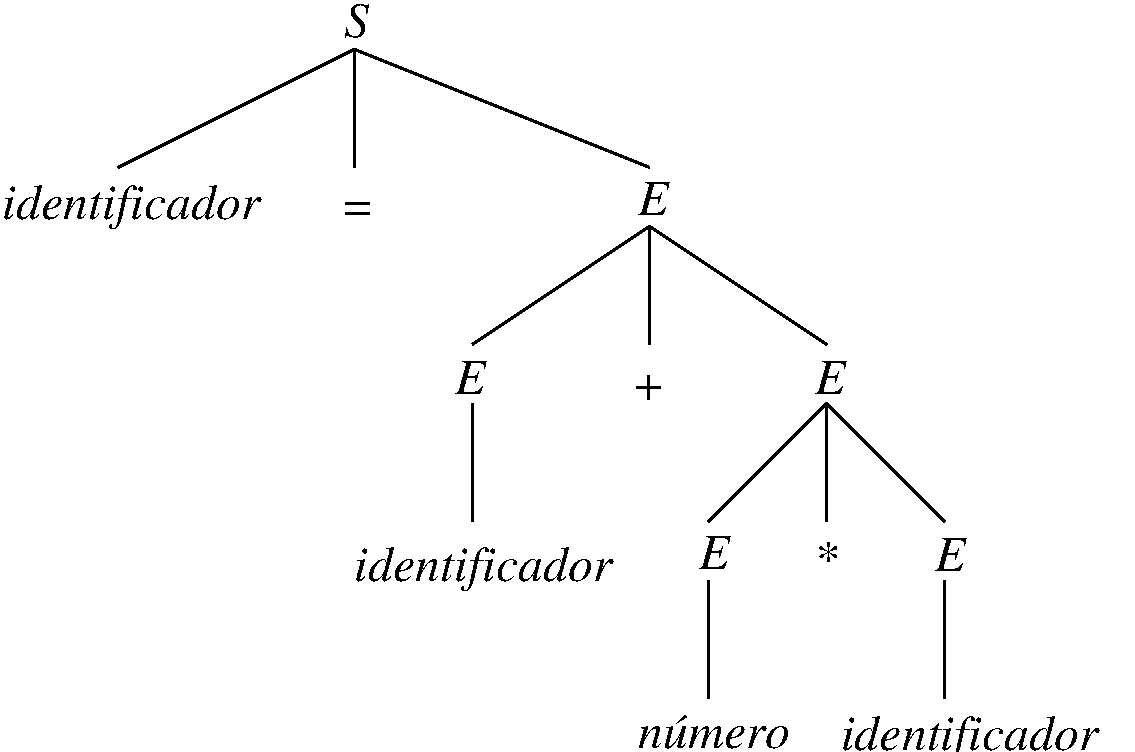
\includegraphics[scale=0.5]{figuras/Cap3/arbol-derivacion-gramatica-contexto-libre.pdf}
 \caption{Ejemplo de árbol sintáctico asociado a una derivación de una gramática de contexto libre.}\label{fig-arbol-derivacion-gramatica-contexto-libre}
\end{figure}


\subsection{Analizadores sintácticos descendentes}\label{sec:descendente}

El análisis sintáctico descendente comprueba si una gramática de contexto libre puede generar la cadena de símbolos de  entrada, como, por ejemplo, una sentencia de un lenguaje de programación, utilizando alguna de las siguientes {\bf estrategias}, que son complementarias:
\begin{itemize}
\item Construcción de una \textbf{derivación por la izquierda} de la cadena de entrada.
\item Construcción de un \textbf{árbol sintáctico} de forma \textbf{descendente} desde la raíz hasta las hojas.
\end{itemize}

Considérese la siguiente gramática que genera sentencias de asignación de expresiones aritméticas:

\begin{eqnarray*}
  P & = & \{ \\
     & (1) & S \longrightarrow \mbox{\bf\em identificador } = \hspace{1ex} E \\
     & (2) & E \longrightarrow T \hspace{1ex} E' \\
     & (3) & E' \longrightarrow + \hspace{1ex} T \hspace{1ex} E' \\
     & (4) & E' \longrightarrow \epsilon \\     
     & (5) & T \longrightarrow F \hspace{1ex} T' \\
     & (6) & T' \longrightarrow * \hspace{1ex} F \hspace{1ex} T' \\
     & (7) & T' \longrightarrow \epsilon \\     
     & (8) & F \longrightarrow ( \hspace{1ex} E \hspace{1ex} ) \\
     & (9) & F \longrightarrow \mbox{\bf\em identificador} \\
     & (10) & F \longrightarrow \mbox{\bf\em número} \\ 
     &   &\}
\end{eqnarray*}

Esta gramática permite generar la siguiente derivación por la izquierda.

\begin{center}
$
\begin{array}{lll}
  S & \Dflecha_1 & {\bf identificador =} \ E \\
   & \Dflecha_2 & {\bf identificador =} \ T E' \\
   & \Dflecha_5 & {\bf identificador =} \ F T' E' \\
   & \Dflecha_9 & {\bf identificador = identificador} T' E' \\
   & \Dflecha_7 & {\bf identificador = identificador \ \epsilon} \  E' \\
   & \Dflecha_3 & {\bf identificador = identificador \ \epsilon \ +} \ T E' \\
   & \Dflecha_5 & {\bf identificador = identificador \ \epsilon \ +} \ F T' E' \\
   & \Dflecha_{10} & {\bf identificador = identificador \ \epsilon \ + n} \ T' E' \\
   & \Dflecha_6 & {\bf identificador = identificador \ \epsilon \ + n \ *} \ F T' E'  \\
   & \Dflecha_9 & {\bf identificador = identificador \ \epsilon \ + n \ * \ identificador} \ T' E' \\
   & \Dflecha_7 & {\bf identificador = identificador \ \epsilon \ + n \ * \ identificador \ \epsilon} \ {E'} \\
   & \Dflecha_4 & {\bf identificador = identificador \ \epsilon \ + n \ * \ identificador \ \epsilon} \ \underline{\epsilon } 
\end{array}
$
\end{center}

Las Figuras \ref{fig:pasos-2-analisis-descendente-predictivo} y \ref{fig:pasos-final-analisis-descendente-predictivo} muestran el paso inicial y final, respectivamente, del árbol sintáctico generado por el análisis descendente. Este árbol invertido ha sido generado de forma descendente desde la raíz hasta la hojas.

\begin{figure}[!t]
    \centering
        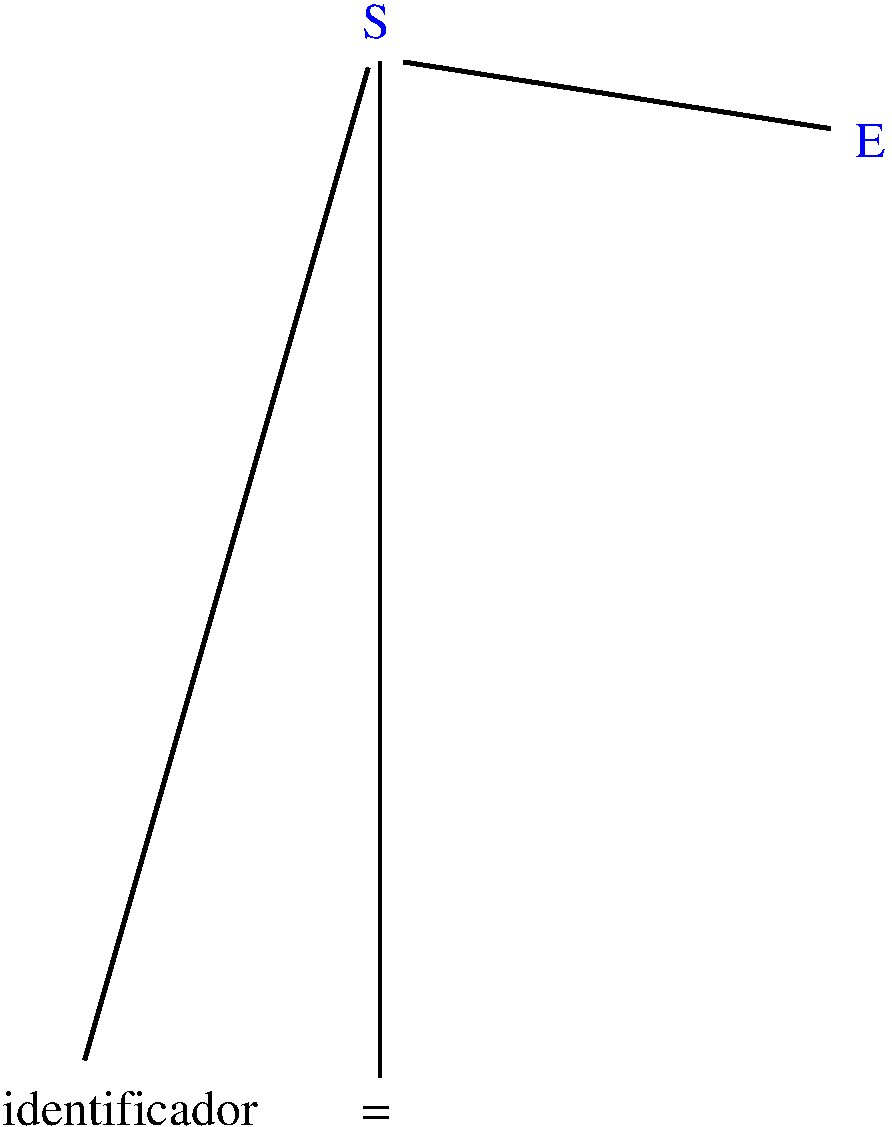
\includegraphics[scale=0.40]{figuras/Cap3/Paso-2-arbol-derivacion-descendente.pdf}
    \caption{Árbol sintáctico: paso inicial del análisis sintáctico descendente predictivo}\label{fig:pasos-2-analisis-descendente-predictivo}
\end{figure}


\begin{figure}[!t]
    \centering
        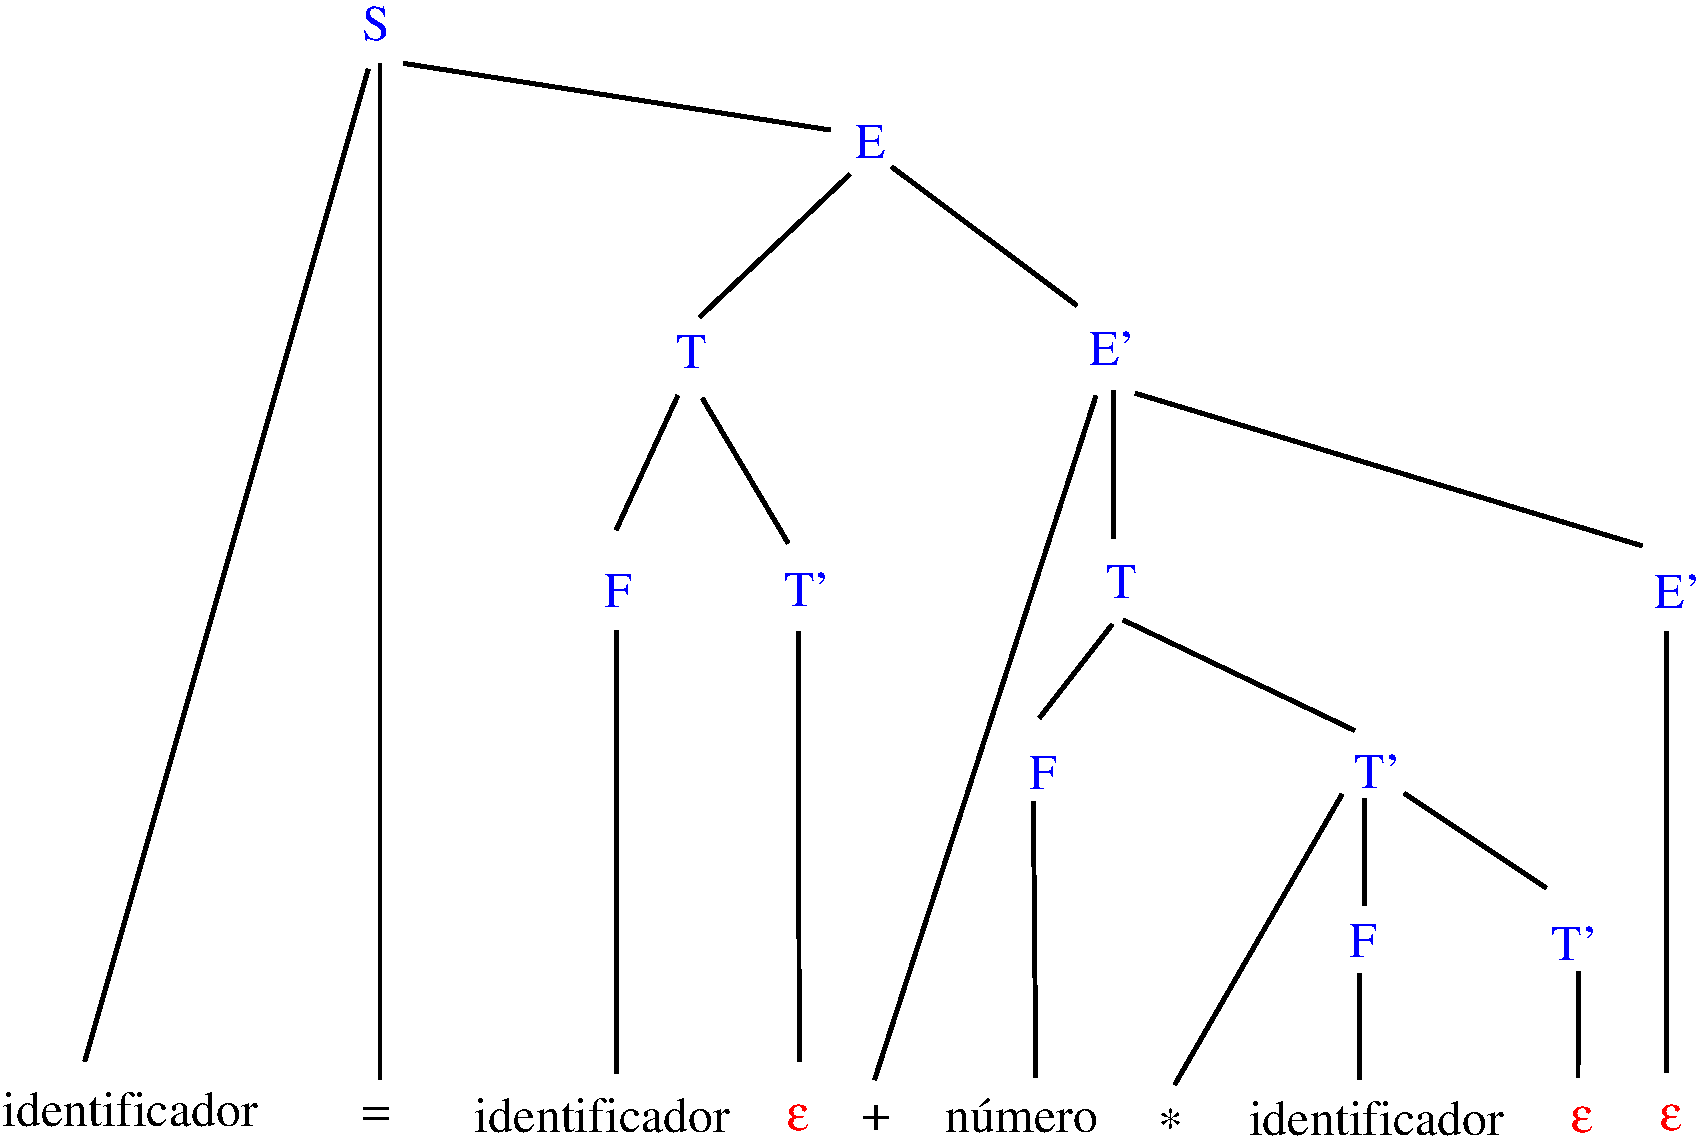
\includegraphics[scale=0.40]{figuras/Cap3/Paso-13-arbol-derivacion-descendente.pdf}
    \caption{Árbol sintáctico: paso final del análisis sintáctico descendente predictivo}\label{fig:pasos-final-analisis-descendente-predictivo}
\end{figure}

Existen diferentes dos tipos de analizadores sintácticos descendentes \cite{aho2008}:
\begin{enumerate}
    \item  Método de descenso recursivo \textbf{con} retroceso o \textit{backtracking}.
    \item Método de descenso \textbf{predictivo}, es decir, \textbf{sin} retroceso.
\end{enumerate}

A su vez, existen dos versiones del análisis descendente predictivo: 
\begin{itemize}
    \item Versión recursiva, que utiliza funciones asociadas a los símbolos no terminales de la gramática de contexto libre.
    \item Versión iterativa, que utiliza una pila para simular el análisis sintáctico descendente.
\end{itemize}

Ambas versiones del análisis descendente predictivo utilizan una \textbf{tabla predictiva} para generar la derivación por la izquierda o el árbol sintáctico de forma descendente.  La Tabla \ref{tabla-analisis-descendente-predictivo} muestra la Tabla de análisis descendente predictivo de la gramática que genera sentencias de asignación de expresiones aritméticas y que se definió previamente.

\begin{table}[htp]
    \centering
    \caption{Tabla de análisis descendente predictivo}
    \label{tabla-analisis-descendente-predictivo}
    \begin{tabular}{|| c || c | c | c | c | c | c | c | c ||} 
      \hline
                  & \multicolumn{8}{c||}{\bf Símbolo de entrada} \\
      \hline 
      \hline 
                  & \textbf{id} & \textbf{=} & \textbf{+} & \textbf{*} & \textbf{(} & \textbf{)} & \textbf{número} & \textbf{\$}  \\ 
      \hline             
      \hline S    &     1       &            &            &            &            &            &                 &  \\ 
      \hline E    &     2       &            &            &            &      2     &            &       2         & \\ 
      \hline E'   &             &            &      3     &            &            &      4     &                 &   4    \\ 
      \hline T    &     5       &            &            &            &      5     &            &       5         &  \\ 
      \hline T'   &             &            &      7     &     6      &            &      7     &                 &  7  \\ 
      \hline F    &     9       &            &            &            &      8     &            &       10        & \\
      \hline
    \end{tabular}
    
\end{table}    

El primer símbolo de cada fila es un símbolo no terminal de la gramática. El primer símbolo de cada columna es o un símbolo terminal de la gramática o el símbolo \$, que representa el fin de la cadena de símbolos que se va a analizar en la entrada. El número que aparece en las celdas interiores de la tabla representa el número de la regla de producción de la gramática que se debe utilizar cuando se está derivando un símbolo no terminal y en la entrada aparece un símbolo terminal o el símbolo \$.

La Tabla \ref{tab:tabla-analisis-descendente-predictivo} muestra cómo se utiliza la Tabla \ref{tabla-analisis-descendente-predictivo} para realizar  el análisis descendente predictivo de la siguiente sentencia:  \textbf{id = id + n * id \$}. La columna \textbf{Acción} de dicha tabla indica las reglas de producción que se deben utilizar para generar la derivación por la izquierda y el árbol sintáctico de forma descendente. Véanse las Figuras \ref{fig:pasos-2-analisis-descendente-predictivo} y \ref{fig:pasos-final-analisis-descendente-predictivo}.

\begin{table}[!t]
\caption{Pasos del análisis descendente predictivo}
    \label{tab:tabla-analisis-descendente-predictivo}
    \centering
\begin{tabular}{l|l|l}
      \hline 
      \textbf{Pila}  \hspace{10ex}                     & \textbf{Entrada}  \hspace{7ex}         & \textbf{Acción} \hspace{8ex}  \\
      \hline 
       {\bf \$} {S}                              & \textbf{ {id} = id + n * id \$}  & 1) S $\rightarrow$ {\bf identificador} {\bf =}  E     \\
       {\bf \$} \underline{E  {\bf =} {\bf id}}  & \textbf{ {id} = id + n * id \$}  & Emparejar   \\
       {\bf \$}  E  {\bf = }                     & \textbf{ {=} id + n * id \$}     & Emparejar   \\
       {\bf \$}  {E}                             & \textbf{ {id} + n * id \$}       & 2) E $\rightarrow$ T E'    \\
       {\bf \$}  \underline{E' {T}}              & \textbf{ {id} + n * id \$}       & 5) T $\rightarrow$ F T'     \\
       {\bf \$}  E' \underline{T' {F}}           & \textbf{ {id} + n * id \$}       & 9) F $\rightarrow$ {\bf identificador}   \\
       {\bf \$}  E' T' \underline{{\bf id}}      & \textbf{ {id} + n * id \$}       & Emparejar \\
       {\bf \$}  E' {T'}                         & \textbf{ {+} n * id \$}          & 7) T' $\rightarrow$ $\epsilon$ \\
       {\bf \$}  {E'}                            & \textbf{ {+} n * id \$}          & 3) E' $\rightarrow$ {\bf +} T E' \\
       {\bf \$} \underline{E' T  {\bf +}}        & \textbf{ {+} n * id \$}          & Emparejar \\
        {{{\bf \$} E' {T}}}  &  {{\textbf{ {n} * id \$}}}     &  \\
        {\bf \$} E' \underline{T' {F}}           &  \textbf{ {n} * id \$}          &  10) F $\rightarrow$ {\bf número} \\
        {\bf \$} E' \underline{T' {\bf n}}       &  \textbf{ {n} * id \$}          & Emparejar  \\
        {\bf \$} E' {T'}                         & \textbf{ {*}  id \$}            & 6) T' $\rightarrow$ {\bf *} F T' \\
        {\bf \$} E' \underline{T' F {\bf *}}     & \textbf{ {*}  id \$}            & Emparejar \\
        {\bf \$} E' T' {F}                       & \textbf{ {id} \$}               &  9) F $\rightarrow$ {\bf identificador} \\
        {\bf \$} E' T' \underline{{\bf id}}      & \textbf{ {id} \$}               &  Emparejar  \\
        {\bf \$} E' {T'}                         & \textbf{ {\$}}                  & 7) T' $\rightarrow$ $\epsilon$ \\
        {\bf \$} {E'}                            & \textbf{ {\$}}                  & 4) E' $\rightarrow$ $\epsilon$ \\
        {\bf \$}                                 & \textbf{ {\$}}                  &  Aceptar\\
       \hline
    \end{tabular}
\end{table}

%\newpage

\subsection{Analizadores sintácticos ascendentes} \label{sec:ascendente}

El análisis sintáctico ascendente comprueba si una gramática de contexto libre puede generar la cadena de símbolos de  entrada, como, por ejemplo, una sentencia de un lenguaje de programación, utilizando alguna de las siguientes {\bf estrategias}, que son complementarias:
\begin{itemize}
\item Construcción de una \textbf{derivación por la derecha en orden inverso} de la cadena de entrada.
\item Construcción de un \textbf{árbol sintáctico} de forma \textbf{ascendente} desde las hojas hasta la raíz.
\end{itemize}


Se han propuesto diferentes métodos de análisis sintáctico ascendente \cite{aho2008}:
\begin{itemize}
 \item Métodos basados en la precedencia
    \begin{itemize}
    \item Métodos de precedencia simple.
    \item Métodos de precedencia débil.
    \item Métodos de precedencia extendida.
    \item Métodos de precedencia de estrategia mixta.
    \item Métodos de precedencia de operadores.
\end{itemize}
 \item Métodos de análisis LR
  \begin{itemize}
      \item Método SLR
      \item Método LR - canónico
      \item Método LALR
  \end{itemize}
\end{itemize}

%En el presente Trabajo de Fin de Grado, solamente se van a considerar los métodos de análisis LR. 
A continuación se muestra un ejemplo de aplicación del método de análisis sintáctico ascendente SLR. Considérese la siguiente gramática de contexto libre que permite generar prototipos de funciones:
\begin{center}
\begin{itemize}
      \item[] {P}  =  \{  
        \begin{itemize}
         \item[(1)] S $\rightarrow$ T {\bf id (} L {\bf ) ;} 
         \item[(2)] T $\rightarrow$ T {\bf *}
         \item[(3)] T $\rightarrow$ {\bf int} 
         \item[(4)] L $\rightarrow$ L {\bf ,} T 
         \item[(5)] L $\rightarrow$ T 
      \end{itemize}
      \item[] \hspace{0.5cm} \}
    \end{itemize}
\end{center}


A partir de esta gramática, se genera la Tabla de análisis sintáctico SLR que se muestra en la Tabla \ref{tab:tabla-SLR}, donde $d$ $n$ indica que se desplaza un símbolo de la entrada a la pila y se pasa al estado $n$; por su parte, $r$ $k$ representa que se utiliza la regla número $k$ de la gramática para reducir el contenido de la cima de la pila al símbolo no terminal de la parte izquierda de la regla $k$. Véase la Tabla \ref{tab:analisis-SLR}.  Una descripción más detallada de este método SLR y de los demás métodos LR se puede consultar en el libro de Aho et al. \cite{aho2008}.

\begin{table}[htp]
    \caption{Tabla de análisis sintáctico SLR}
    \label{tab:tabla-SLR}
    \centering
    \begin{tabular}{| c | c | c | c | c | c | c | c | c || c | c | c |}
      \hline \multicolumn{8}{|c}{\bf Acción} & &\multicolumn{3}{c|}{\bf Ir-a}  \\
      \hline                   & \textbf{id} & \textbf{(} & \textbf{)} & \textbf{;} & \textbf{*} & \textbf{int}                  & \textbf{,} & \textbf{\$} & \textbf{S} & \textbf{T} & \textbf{L} \\ 
      \hline \hline \textbf{0} &             &            &            &            &            & \textbf{d 3} &            &              & \textbf{1} & \textbf{2} & \\ 
      \hline \textbf{1}        &             &            &            &            &            &                               &            & \textbf{Aceptar}         &  &  & \\ 
      \hline \textbf{2}        & \textbf{d 4} &  &  &  & \textbf{d 5} & & & & & & \\ 
      \hline \textbf{3}        & \textbf{r 3} &  & \textbf{r 3} &  & \textbf{r 3} & & \textbf{r 3} & & & & \\
      \hline \textbf{4}        &  & \textbf{d 6} &  &  & & & & & & & \\ 
      \hline \textbf{5}        & \textbf{r 2} &  & \textbf{r 2} &  & \textbf{r 2} & & \textbf{r 2} & & & & \\
      \hline \textbf{6}        &  &  &  &  & & \textbf{d 3} & & & & \textbf{8} & \textbf{7} \\ 
      \hline \textbf{7}        &  &  & \textbf{d 9} &  & &  & \textbf{d 10} & & & &  \\ 
      \hline \textbf{8}        &  &  & \textbf{r 5} &  & \textbf{d 5}  &  & \textbf{r 5} & & & & \\
      \hline \textbf{9}        &  &  &  & \textbf{d 11} &   &  & & & & & \\
      \hline \textbf{10}       &             &             &           &             &            &  \textbf{d 3}  &  &  &  & \textbf{12} & \\ 
      \hline \textbf{11}       &  &  &  &  &   &  & & \textbf{r 1} & & & \\
      \hline \textbf{12}       &  &  & \textbf{r 4} &  & \textbf{d 5} &  & \textbf{r 4} &  & & & \\
      \hline
    \end{tabular}
\end{table}


\begin{table}[htp]
    \caption{Pasos del análisis sintáctico ascendente SLR}
    \label{tab:analisis-SLR}
    \centering
    \begin{tabular}{l|l|l}
      \hline \hline \textbf{Pila}                & \textbf{Entrada}                                 & \textbf{Acción} \\
      \hline 
      0                       & \textbf{{int} id ( int ) ;} \$ & desplazar 3  \\
      0 \underline{{\bf int} 3}  & \textbf{id ( int ) ;} \$       & reducir 3) T $\rightarrow$ {\bf int} \\
      0 T 2  & \textbf{id ( int ) ;} \$       & desplazar 4 \\
      0 T 2 {\bf id} 4    & \textbf{( int ) ;} \$       & desplazar 6 \\
      0 T 2 {\bf id} 4 {\bf (} 6  & \textbf{int ) ;} \$           & desplazar 3 \\
      0 T 2 {\bf id} 4 {\bf (} 6 \underline{{\bf int} 3} & \textbf{) ;} \$    & reducir 3) T $\rightarrow$ {\bf int} \\
      0 T 2 {\bf id} 4 {\bf (} 6 \underline{{\bf int} 3}               & \textbf{) ;} \$  & reducir 3) T $\rightarrow$ {\bf int} \\
      0 T 2 {\bf id} 4 {\bf (} 6 \underline{T 8}                       & \textbf{) ;} \$  & reducir 5) L $\rightarrow$ T\\
      0 T 2 {\bf id} 4 {\bf (} 6 L 7                                   & \textbf{) ;} \$  & desplazar 9  \\
      0 T 2 {\bf id} 4 {\bf (} 6 L 7 {\bf )} 9  & \textbf{;} \$    & desplazar 11\\
      0 \underline{T 2 {\bf id} 4 {\bf (} 6 L 7 {\bf )} 9 {\bf ;} 11}  & \textbf{\$}   & reducir 1) S $\rightarrow$ T {\bf id (} L {\bf ) ;}\\
      0 S 1  & \textbf{\$}      & \textbf{Aceptar}\\
      \hline
    \end{tabular}

\end{table}


Usando la Tabla \ref{tab:tabla-SLR}, se pueden realizar los pasos del análisis sintáctico ascendente que se muestran en la Tabla \ref{tab:analisis-SLR} y que permiten generar la derivación por la derecha de que se indica a continuación:
\begin{center}
\begin{tabular}{lcl}
     {S} & $\Dflecha_{1}$ & \underline{T {\bf id (} {L} {\bf ) ;}} \\
               & $\Dflecha_{5}$ & T {\bf id (} \underline{{T}} {\bf ) ;} \\
               & $\Dflecha_{3}$ & {T} {\bf id ( \underline{int} ) ;} \\
               & $\Dflecha_{3}$ & {\bf \underline{int} id ( int ) ;}
 \end{tabular}
\end{center}

La Figura \ref{fig:pasos-analisis-ascendente-SLR} muestra el paso inicial y final de la generación del árbol sintáctico (invertido) construido de forma ascendente desde las hojas hasta la raíz.

\begin{figure}[htp]
    \centering
    \begin{tabular}{c}
        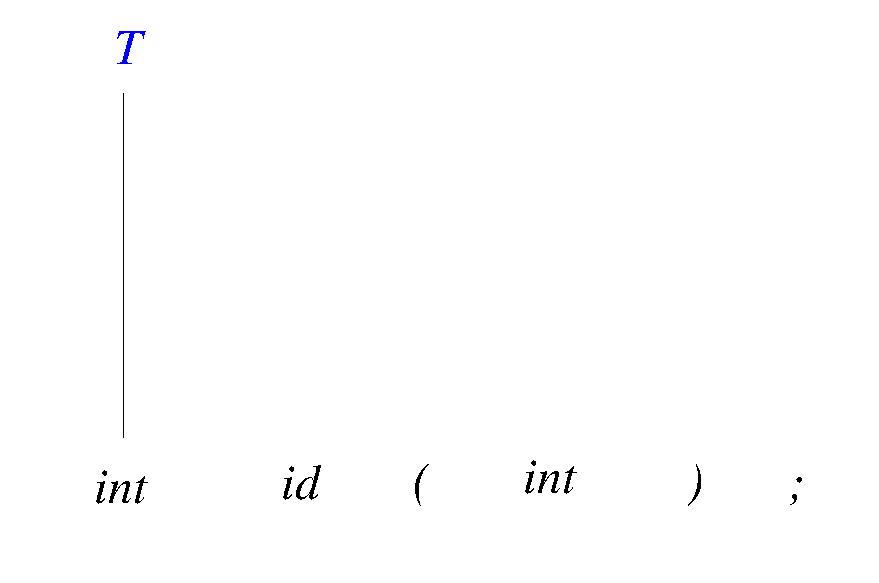
\includegraphics[scale=0.5]{figuras/Cap3/SLR-paso-inicial.pdf} \\ 
        (a) \\ 
        \\
        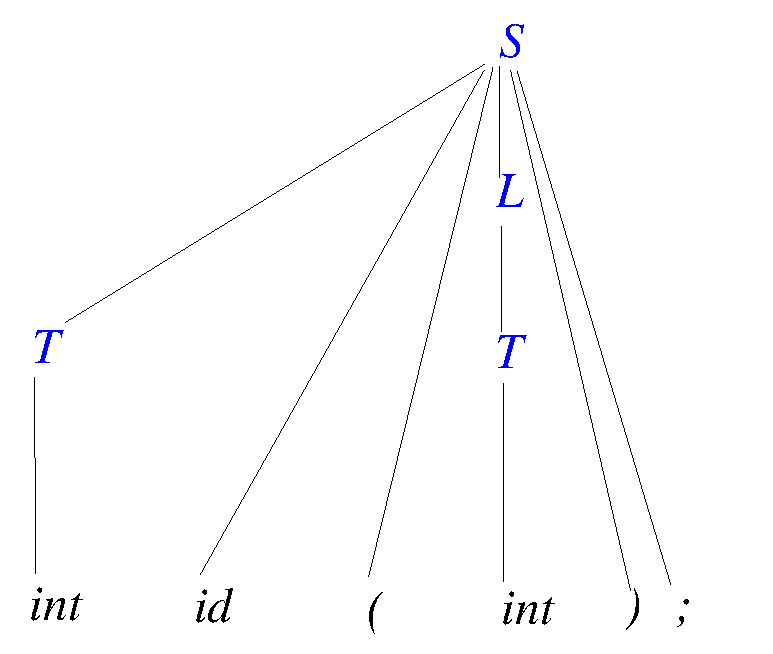
\includegraphics[scale=0.5]{figuras/Cap3/SLR-paso-final.pdf}  \\
        (b)
    \end{tabular}
    \caption{Árbol sintáctico: pasos (a) inicial y (b) final del análisis sintáctico ascendente SLR}\label{fig:pasos-analisis-ascendente-SLR}
\end{figure}

\newpage 

\section{SimAS 1.0}\label{sec:SimAs1.0}

Este Trabajo de Fin de Grado se centra en el desarrollo de un simulador de analizadores sintácticos descendentes, habiendo existido una primera versión previa denominada SimAs 1.0 \cite{vanesa}, la cuál fue posteriormente mejorada. En esta sección, se describen las características principales de dicha versión inicial, la cual servirá como referencia para el desarrollo de la nueva versión.

SimAs 1.0. es una aplicación de escritorio y multiplataforma desarrollada en 2015 con los siguientes recursos de software:
 \begin{itemize}
     \item Sistemas operativos: Ubuntu Linux (versión 12.10) \cite{ubuntu} y Microsoft Windows 7 \cite{windows}.
     \item Lenguaje de programación: Java SE (JDK) 7u40 \cite{java}.
     \item Entorno de desarrollo: NetBeans 7.3.1. \cite{netbeans}.
     \item Biblioteca para la interfaz gráfica: Java Swing \cite{javaswing}.
     \item Biblioteca iText 5.5.0 de Java para la generación de informes en formato pdf \cite{itextpdf}.
     \item XML \cite{xml}: formato utilizado para almacenar las gramáticas formales.
 \end{itemize}

En las siguientes figuras, se describen algunas de las características más importantes del funcionamiento de la versión 1.0 de SimAs. 

 \begin{figure}[!t]
 	\begin{center}
      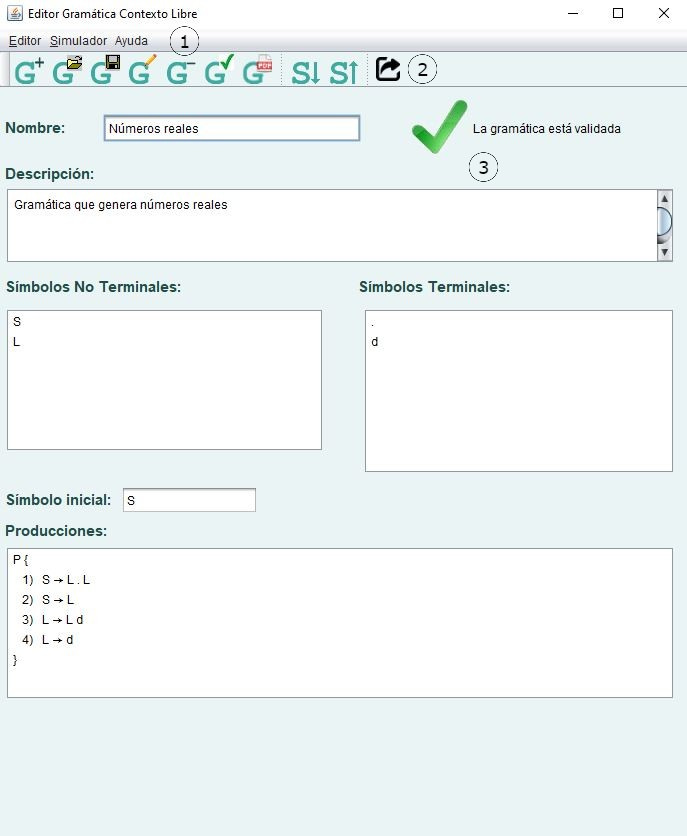
\includegraphics[scale=0.5]{figuras/Cap3/interfaz.JPG} 
       \caption{Interfaz del editor de SimAS 1.0.}\label{fig:SimAS-1.0-editor}
 	\end{center}
 \end{figure}


La figura \ref{fig:SimAS-1.0-editor} muestra la interfaz del editor de SimAS 1.0. En dicha figura, se han numerado algunos componentes que son descritos a continuación:
 \begin{enumerate}
     \item Se muestra la barra de menús donde se puede escoger entre opciones: editor, simulador o ayuda.
     \item La barra de herramientas permite acceder rápidamente a las opciones más frecuentes, como crear abrir o guardar una gramática, verificarla o incluso escoger entre si se prefiere usar el análisis ascendente o descendente.
     \item El editor está compuesto por diferentes formularios para indicar el nombre de la gramática, añadir una pequeña descripción, sus  símbolos terminales y no terminales, establecer el símbolo inicial y definir sus reglas de producción
 \end{enumerate}


 \begin{figure}[!t]
   \begin{center}
      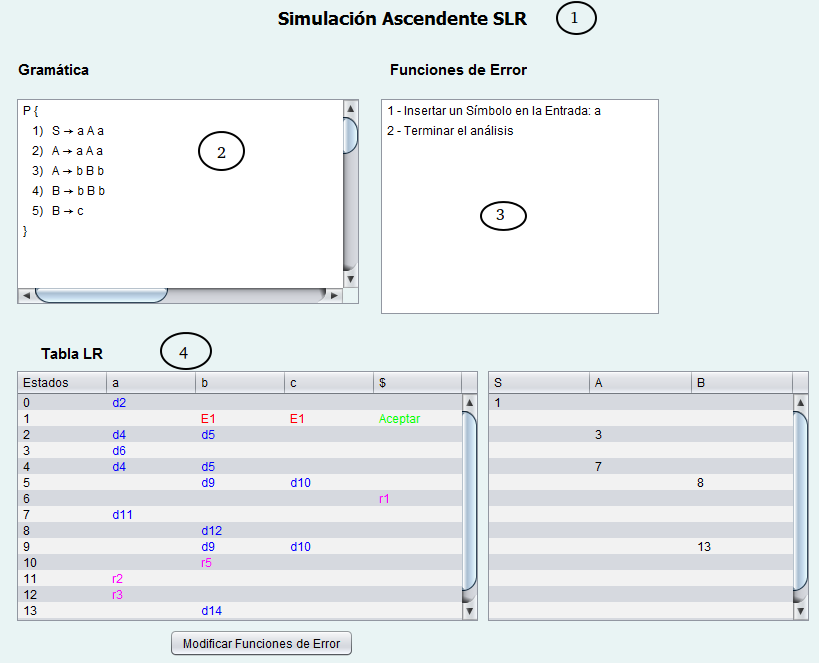
\includegraphics[scale=0.40]{figuras/Cap3/da12.png} 
       \caption{Panel del editor de SimAS 1.0 }\label{fig:SimAS-1.0-editor-funciones-de-error}
 	\end{center}
   \end{figure}

La figura \ref{fig:SimAS-1.0-editor-funciones-de-error} muestra cómo se pueden asignar funciones de tratamiento de errores en el método SLR de análisis sintáctico ascendente. Los componentes numerados se describen a continuación:
\begin{enumerate}
     \item Se indica el tipo de simulación que se llevará a cabo.
     \item Se muestra la gramática de contexto libre que se va a utilizar.
     \item Funciones de tratamiento de errores que se pueden utilizar en  la simulación del análisis sintáctico.
     \item Tabla de análisis LR
\end{enumerate}

\begin{figure}[!t]
 	\begin{center}
      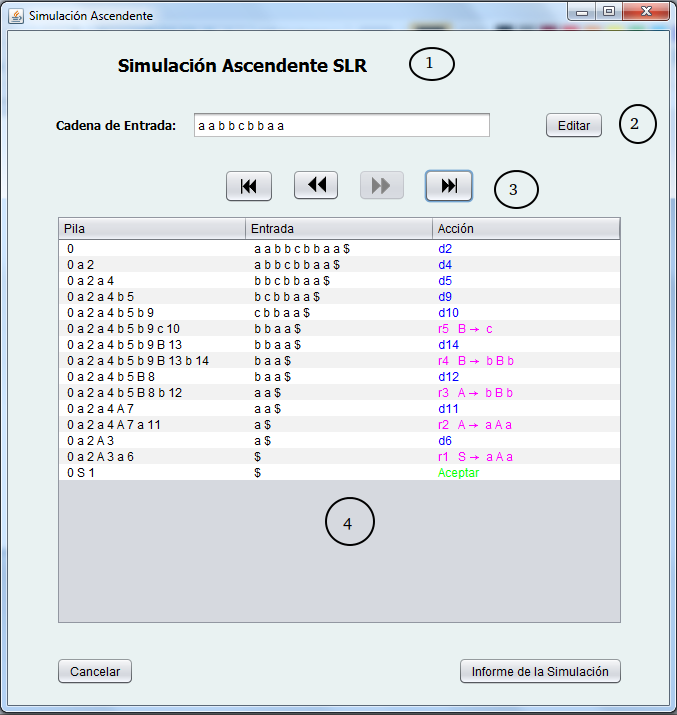
\includegraphics[scale=0.40]{figuras/Cap3/da14.png} 
       \caption{Ventana del simulador de SimAS 1.0.}\label{fig:SimAS-1.0-simulador}
 	\end{center}
\end{figure}

Por último, la figura \ref{fig:SimAS-1.0-simulador} muestra la ventana para la simulación del método SLR de análisis sintáctico ascendente:
\begin{enumerate}
     \item Se indica el tipo de simulación que se va a realizar: simulación ascendente SLR.
     \item Formulario para introducir y editar una cadena de entrada para poder realizar la simulación.
     \item Se muestran una serie de flechas que permiten reproducir la simulación hacia adelante, hacia atrás, etc.
     \item En este último apartado, se muestran los resultados de la simulación.
\end{enumerate}


\section{SimAS 2.0}\label{sec:SimAs2.0}

SimAS 2.0 \cite{juan} se desarrolló para corregir y ampliar la versión de SimAS 1.0 \cite{vanesa}. SimAS 1.0 se instaló en diferentes equipos y se comprobó que permitía simular el funcionamiento de los analizadores sintácticos descendentes y ascendentes. Sin embargo, se detectaron algunos fallos y limitaciones que se intentaron corregir con mejoras que se enumeran a continuación:
\begin{enumerate}
     \item Mejorar el almacenamiento de las gramáticas de contexto libre en formato XML. 
         \begin{itemize}
         \item Procesar de forma individualizada los símbolos de la parte derecha de una regla de producción.
         \item Al cargar una gramática, respetar el orden de sus reglas de producción. No se respeta si ya hay otra gramática previamente cargada.
         \end{itemize}
     \item Validar la gramática cuando se cargue o se modifique, es decir, comprobar que no tiene símbolos y reglas inútiles. En la versión anterior, se debía pulsar un botón para validar.
     \item Al eliminar la recursividad por la izquierda o factorizar por la izquierda, permitir que se pueda conservar la gramática original y la nueva gramática. Además, también debe permitir la enumeración de las reglas de producción de la nueva gramática.
     \item Permitir que la gramática que se está procesando se pueda mostrar o consultar en cualquier momento de forma simultánea en cualquier paso del proceso de simulación de los analizadores sintácticos.
     \item Al construir los conjuntos Primero y Siguiente, mostrar las dependencias entre los conjuntos.
     \item Simular correctamente las gramáticas con reglas épsilon. En particular, calcular correctamente el conjunto Primero en gramáticas reglas épsilon.
     \item Crear funciones predefinidas de recuperación de errores en las simulaciones de los analizadores sintácticos. 
     \item Permitir que se puedan completar las celdas vacías de la tabla de análisis sintáctico descendente con reglas épsilon, cuando proceda, sin tener que predefinir funciones de error.
     \item Permitir que se puedan completar las celdas vacías de la tabla de análisis sintáctico ascendente con reducciones, cuando proceda, sin tener que predefinir funciones de error.
     \item Mostrar las derivaciones obtenidas por los analizadores sintácticos.
     \item Permitir la generación de informes en formato pdf. La aplicación SimAS podía generar estos informes, pero la actualización del sistema operativo no lo permite ahora.
\end{enumerate}

Además, se intentó que la nueva versión  SimAS 2.0 permitiese la generación ``paso a paso'' de los árboles sintácticos de las derivaciones generadas al simular los analizadores sintácticos descendentes o ascendentes.


En su momento, se consideró que el desarrollo de la versión 2.0 estaba justificado por las siguientes razones:
\begin{itemize}
     \item La nueva versión del simulador SimAS 2.0 sería de gran ayuda para que los estudiantes pudiesen aprender ``paso a paso'' el funcionamiento de los analizadores sintácticos descendentes y ascendentes.
     \item La corrección de los errores de SimAS 1.0 evitará que los estudiantes puedan cometerlos.
     \item La inclusión de la generación de los árboles sintácticos asociados a las derivaciones permitiría que los estudiantes comprendan mejor el funcionamiento de los analizadores sintácticos.
\end{itemize}

En las siguientes figuras, se describen algunas de las características más importantes del funcionamiento de la versión 2.0 de SimAS.
 
\begin{figure}[p]
 	\begin{center}
      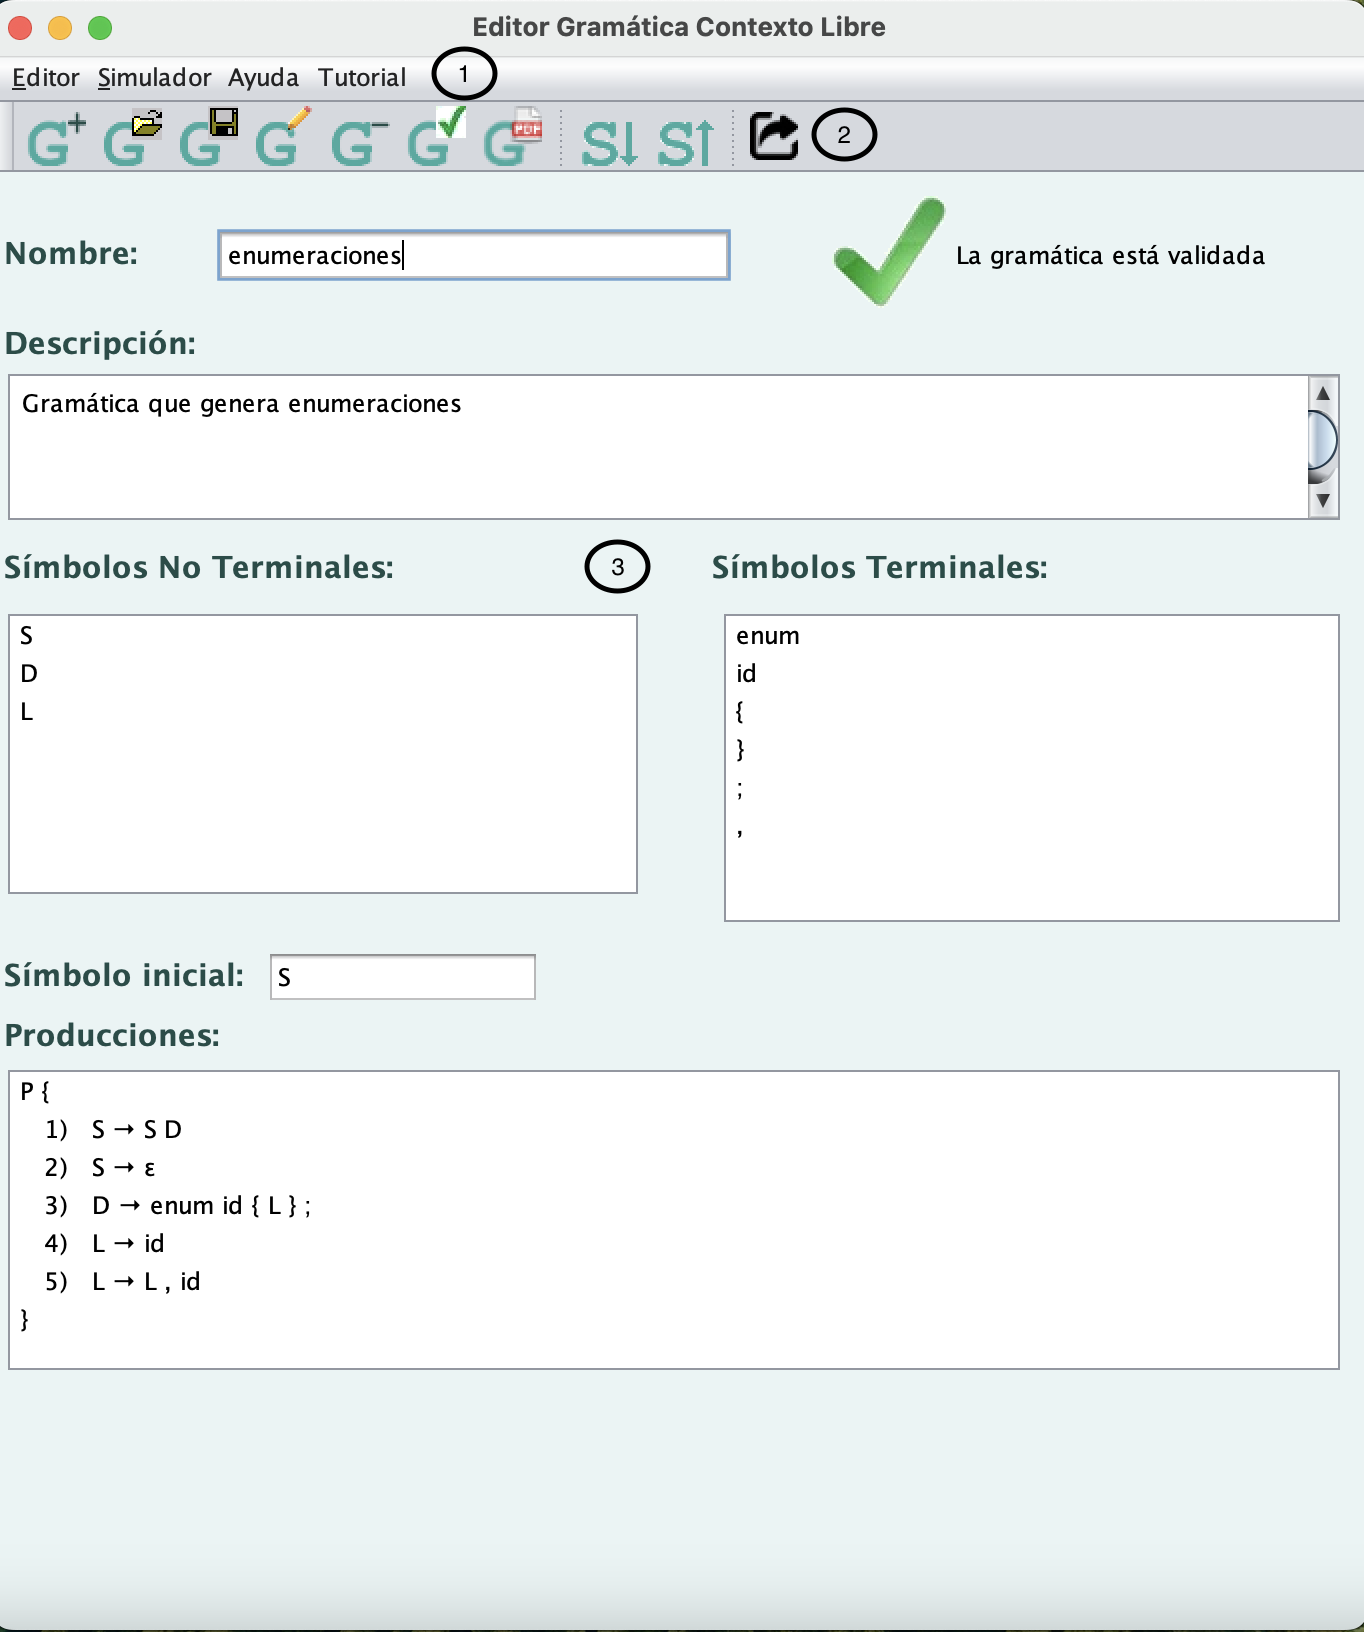
\includegraphics[scale=0.5]{figuras/Cap3/SimAS2/editor.png} 
       \caption{Interfaz del editor de SimAS 2.0.}\label{fig:SimAS-2.0-editor}
 	\end{center}
\end{figure}


La figura \ref{fig:SimAS-2.0-editor} muestra la interfaz del editor de SimAS 2.0, la cual contiene pocas variaciones respecto a la versión original. En dicha figura, se han numerado algunos componentes que son descritos a continuación:
 \begin{enumerate}
     \item La interfaz presenta una barra de menús que brinda opciones como editor, simulador, ayuda y un tutorial detallado para comprender su funcionamiento.
     \item Además, la barra de herramientas facilita el acceso a las funciones más utilizadas, como la creación, apertura y guardado de gramáticas, así como la verificación de las mismas. También permite elegir entre el análisis ascendente y el descendente.
     \item En cuanto al editor, se compone de distintos formularios que permiten especificar el nombre de la gramática, agregar una breve descripción, definir los símbolos terminales y no terminales, establecer el símbolo inicial y definir las reglas de producción.
 \end{enumerate}

\begin{figure}[p]
 	\begin{center}
      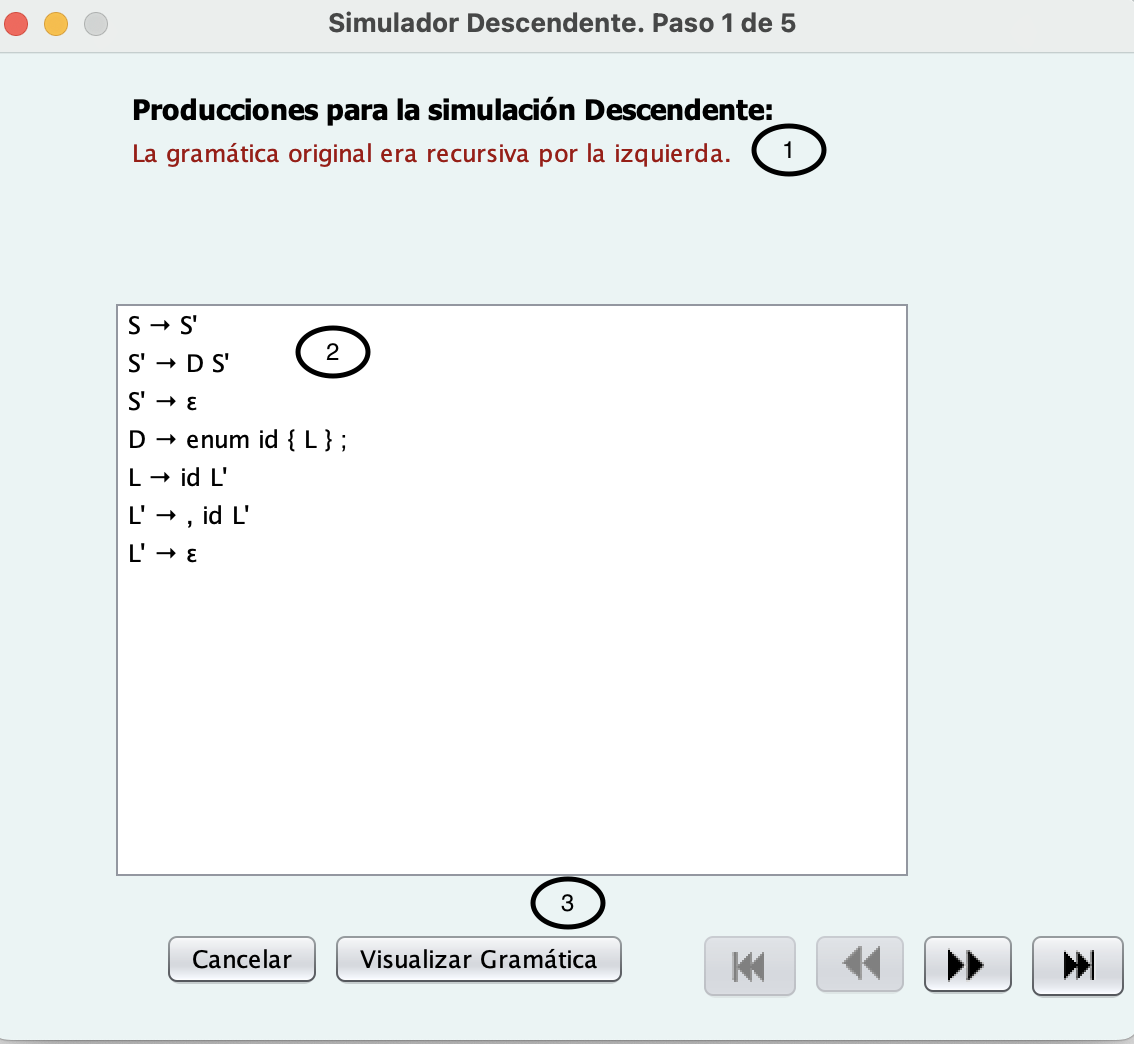
\includegraphics[scale=0.5]{figuras/Cap3/SimAS2/paso1.png} 
       \caption{Corrección de gramáticas de SimAS 2.0.}\label{fig:SimAS-2.0-paso1}
 	\end{center}
\end{figure}


La figura \ref{fig:SimAS-2.0-paso1} muestra el primer paso a realizar para el análisis de gramáticas en SimAS 2.0, que consiste en la eliminación de recursividad de la gramática original. En dicha figura, se han numerado algunos componentes que son descritos a continuación:
 \begin{enumerate}
     \item En primer lugar, aparece un mensaje indicativo con los cambios realizados a la gramática original.
     \item En segundo lugar, se muestra la nueva gramática generada tras realizar los cambios oportunos a la gramática original.
     \item Además, nos da la opción de consultar la gramática original para poder comparar ambas gramáticas.
 \end{enumerate}

 \begin{figure}[p]
 	\begin{center}
      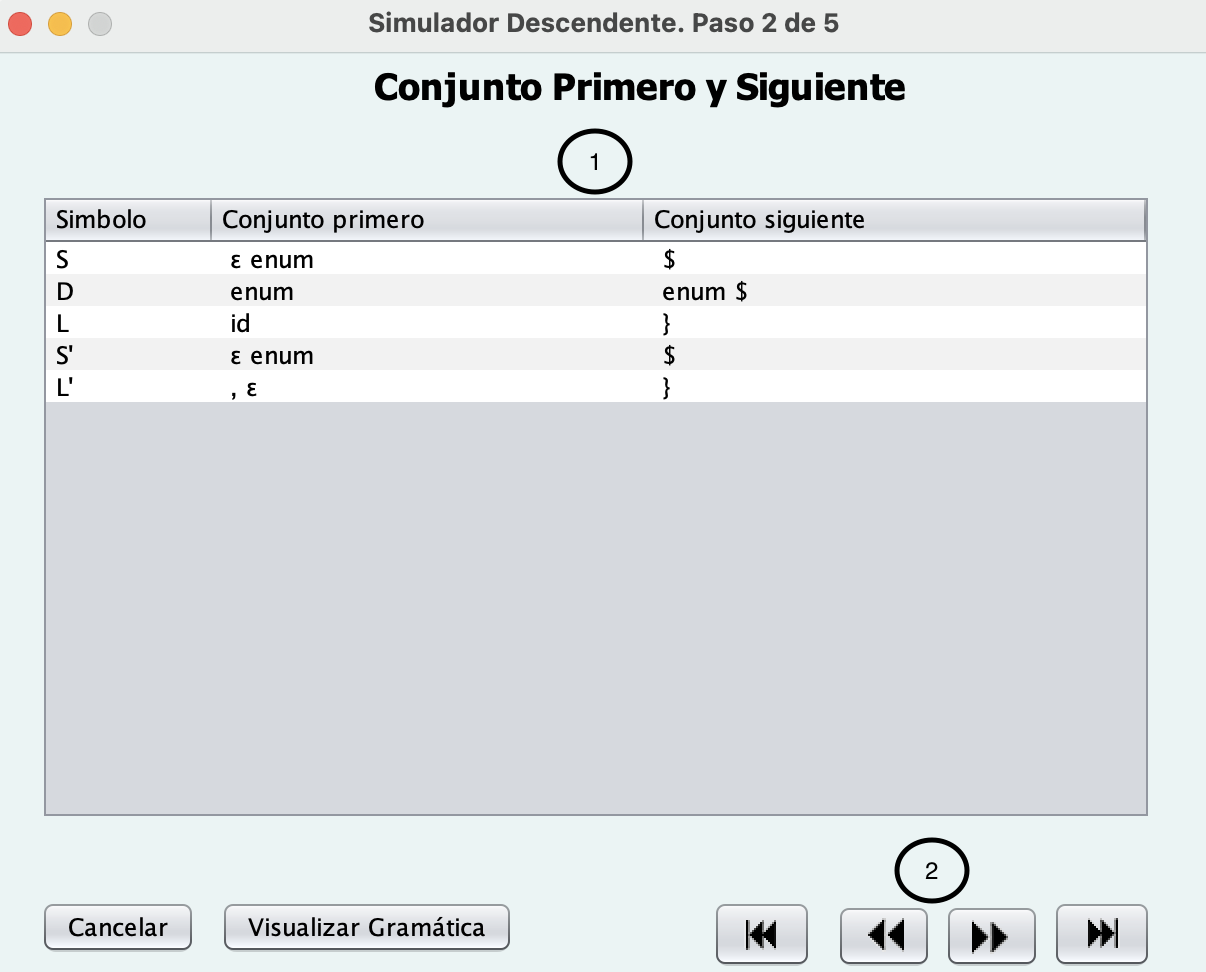
\includegraphics[scale=0.5]{figuras/Cap3/SimAS2/paso2.png} 
       \caption{Conjunto Primero y Siguiente de SimAS 2.0.}\label{fig:SimAS-2.0-paso2}
 	\end{center}
\end{figure}

\newpage
La figura \ref{fig:SimAS-2.0-paso2} muestra los conjuntos Primero y Siguiente generados para el análisis de gramáticas en SimAS 2.0. En dicha figura, se han numerado algunos componentes que son descritos a continuación:
 \begin{enumerate}
     \item El usuario puede ver una tabla con los conjuntos Primero y Siguiente correspondientes a cada símbolo no terminal.
     \item También tenemos un menú común a todos los pasos, que anteriormente no se había mencionado, que permite avanzar paso a paso o  avanzar directamente al último paso.
 \end{enumerate}

\begin{figure}[htp]
 	\begin{center}
      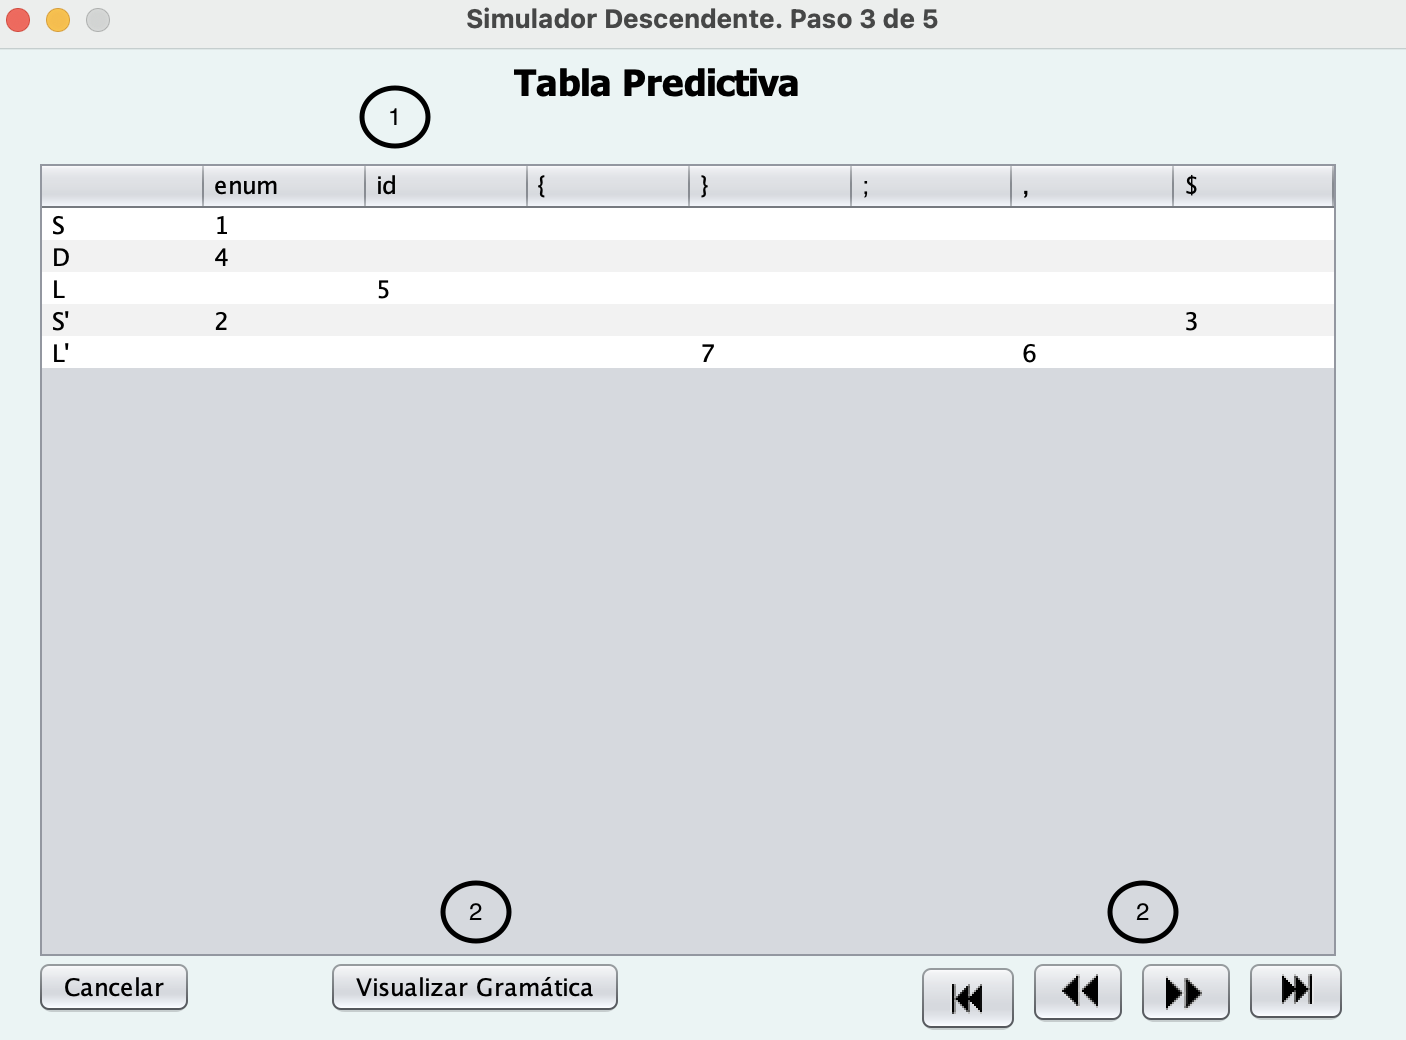
\includegraphics[scale=0.5]{figuras/Cap3/SimAS2/paso3.png} 
       \caption{Tabla predictiva de SimAS 2.0.}\label{fig:SimAS-2.0-paso3}
 	\end{center}
\end{figure}

La figura \ref{fig:SimAS-2.0-paso3} muestra la tabla predictiva generada por el análisis de gramáticas en SimAS 2.0. En dicha figura, se han numerado algunos componentes que son descritos a continuación:
 \begin{enumerate}
     \item En primer lugar, la interfaz contiene la tabla predictiva generada por el programa para la gramática.
     \item Al igual que en el resto de pasos intermedios, el programa contiene la posibilidad de visualizar la gramática original, y el menú de avance y retroceso.
 \end{enumerate}

 \begin{figure}[htp]
 	\begin{center}
      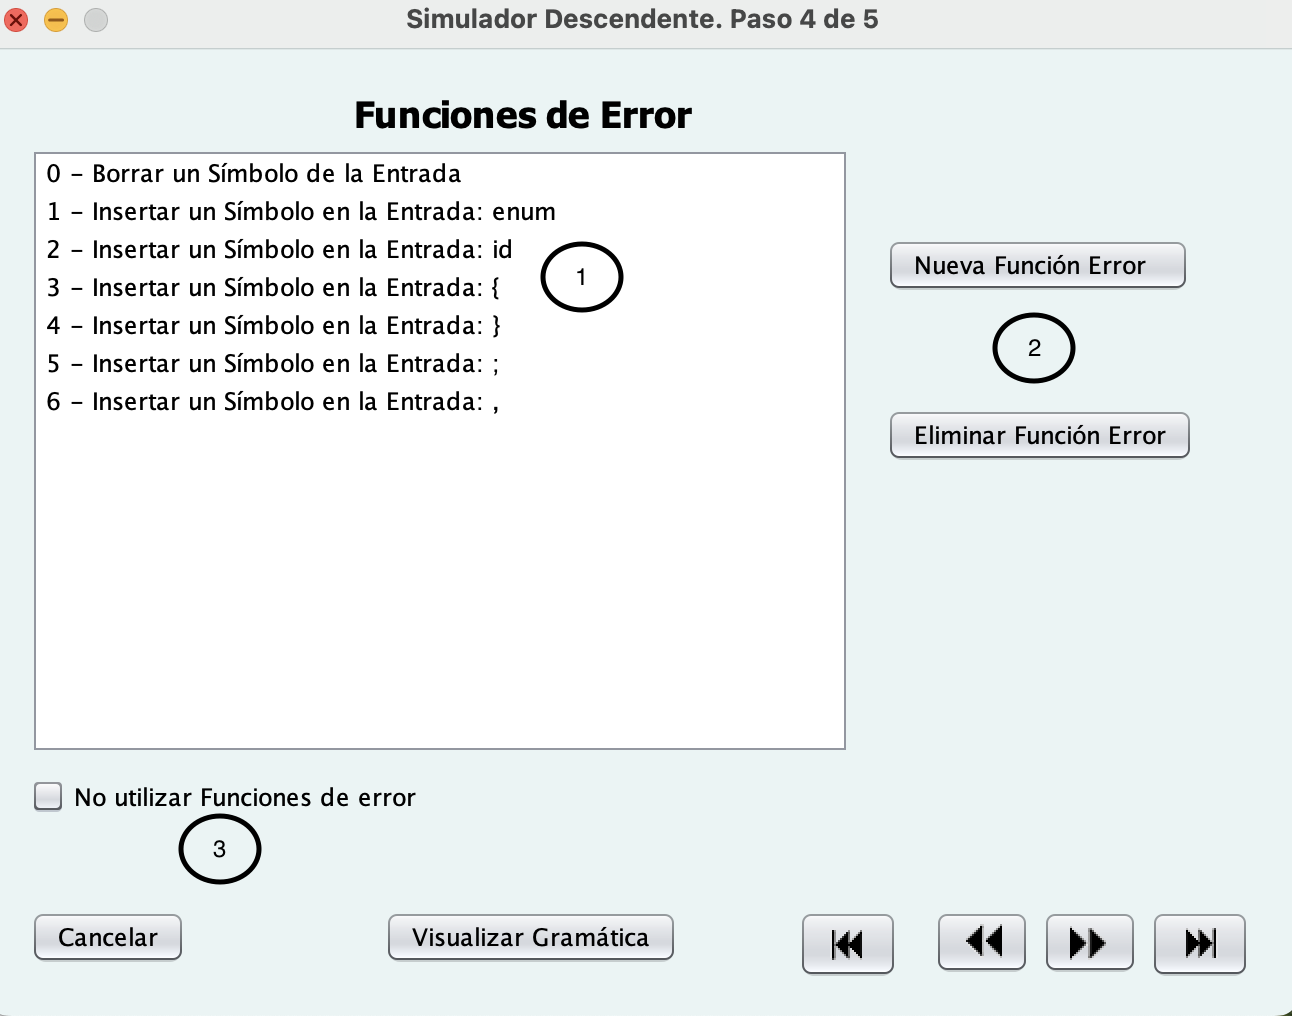
\includegraphics[scale=0.5]{figuras/Cap3/SimAS2/paso4.png} 
       \caption{Tabla predictiva de SimAS 2.0.}\label{fig:SimAS-2.0-paso4}
 	\end{center}
\end{figure}

La figura \ref{fig:SimAS-2.0-paso4} muestra las funciones de error predefinidas o que podemos definir respecto para las gramáticas en SimAS 2.0. En dicha figura, se han numerado algunos componentes que son descritos a continuación:
 \begin{enumerate}
     \item En primer lugar, podemos ver las gramáticas predefinidas que contiene el programa, que comparando con la versión anterior, vemos que son muchas más.
     \item Además, un cambio importante respecto a la versión anterior, es que ésta da la posibilidad de añadir o eliminar funciones de error directamente desde esta interfaz.
     \item Otro cambio significativo respecto a la versión anterior es que se da la opción de no usar funciones de error, lo que hace que el programa salte directamente a la parte final, sin pasar por el paso 5.
 \end{enumerate}

\begin{figure}[htp]
 	\begin{center}
      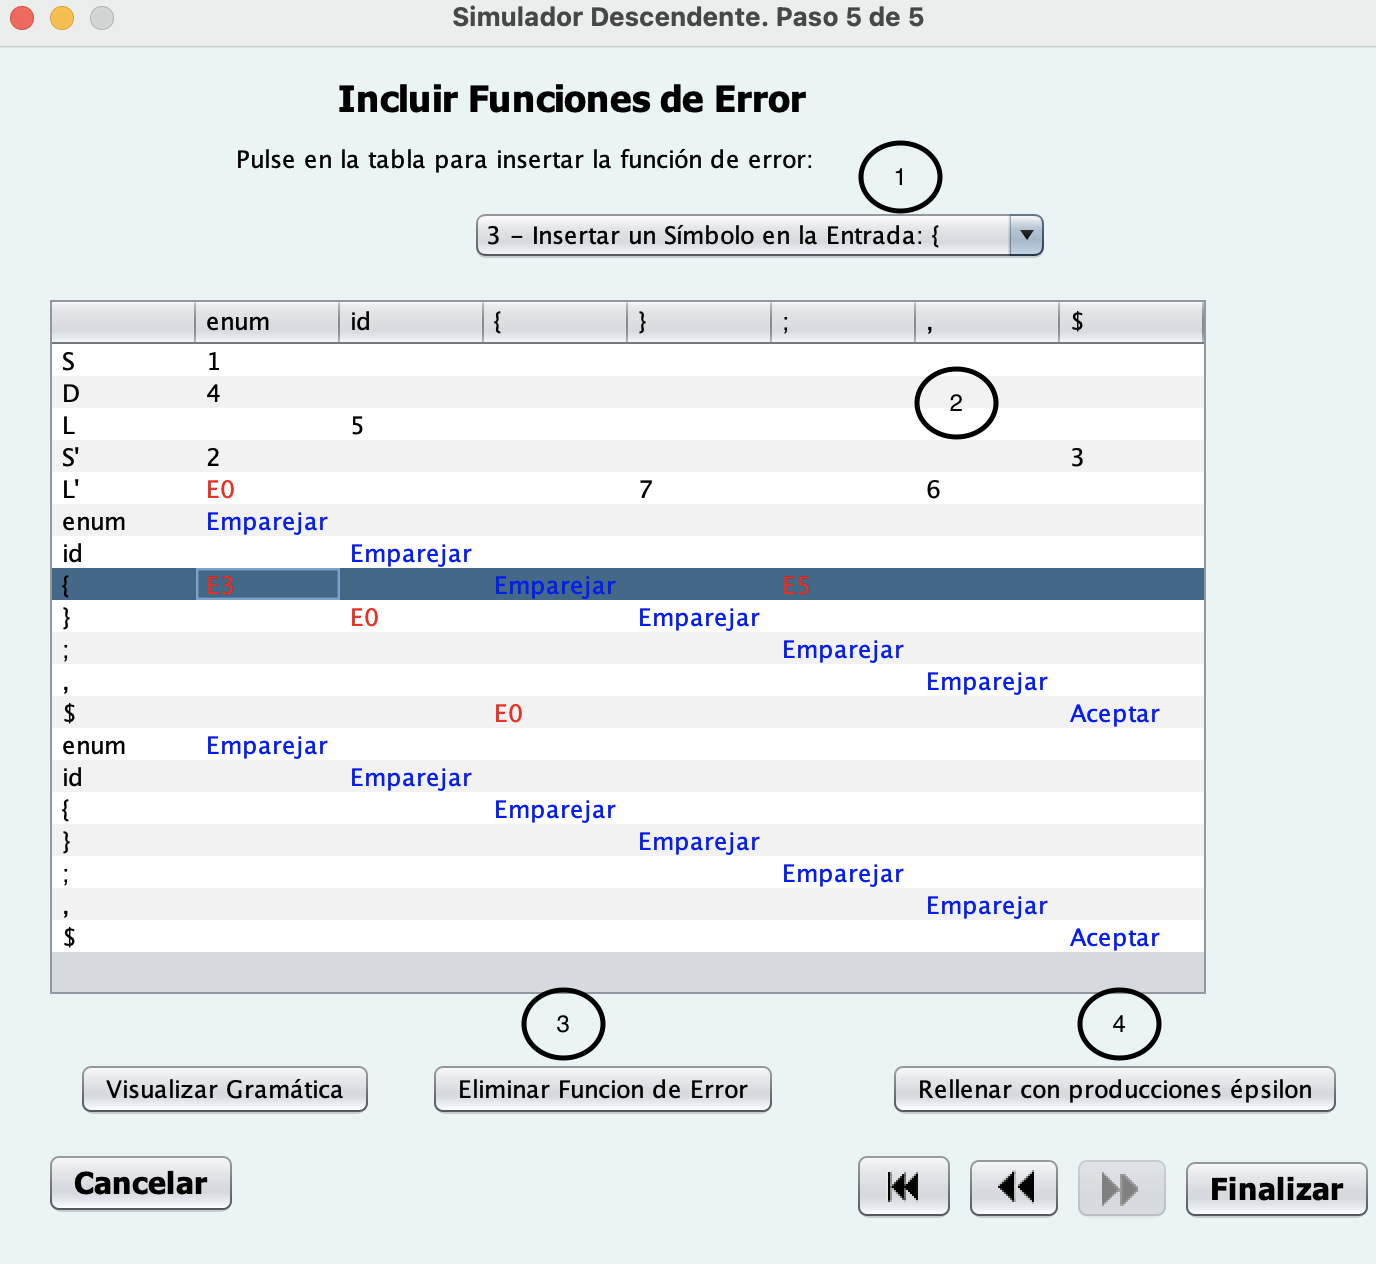
\includegraphics[scale=0.5]{figuras/Cap3/SimAS2/paso5.png} 
       \caption{Tabla predictiva con funciones de errores de SimAS 2.0.}\label{fig:SimAS-2.0-paso5}
 	\end{center}
\end{figure}

La figura \ref{fig:SimAS-2.0-paso5} muestra las funciones de error predefinidas o que podemos definir respecto para las gramáticas en SimAS 2.0. En dicha figura, se han numerado algunos componentes que son descritos a continuación:
 \begin{enumerate}
     \item En primer lugar, se ofrece un menú con las funciones de error definidas en el paso anterior.
     \item En segundo lugar, se tiene la tabla predictiva aumentada para que el usuario añada dichas funcionas de forma intuitiva y muy rápida.
     \item Se añade la opción de eliminar alguna función de error que el usuario estime como incorrecta.
     \item Finalmente, el programa da la opción de rellenar la tabla con las producciones épsilon que pertenezcan a dicha gramática.
 \end{enumerate}

\begin{figure}[htp]
 	\begin{center}
      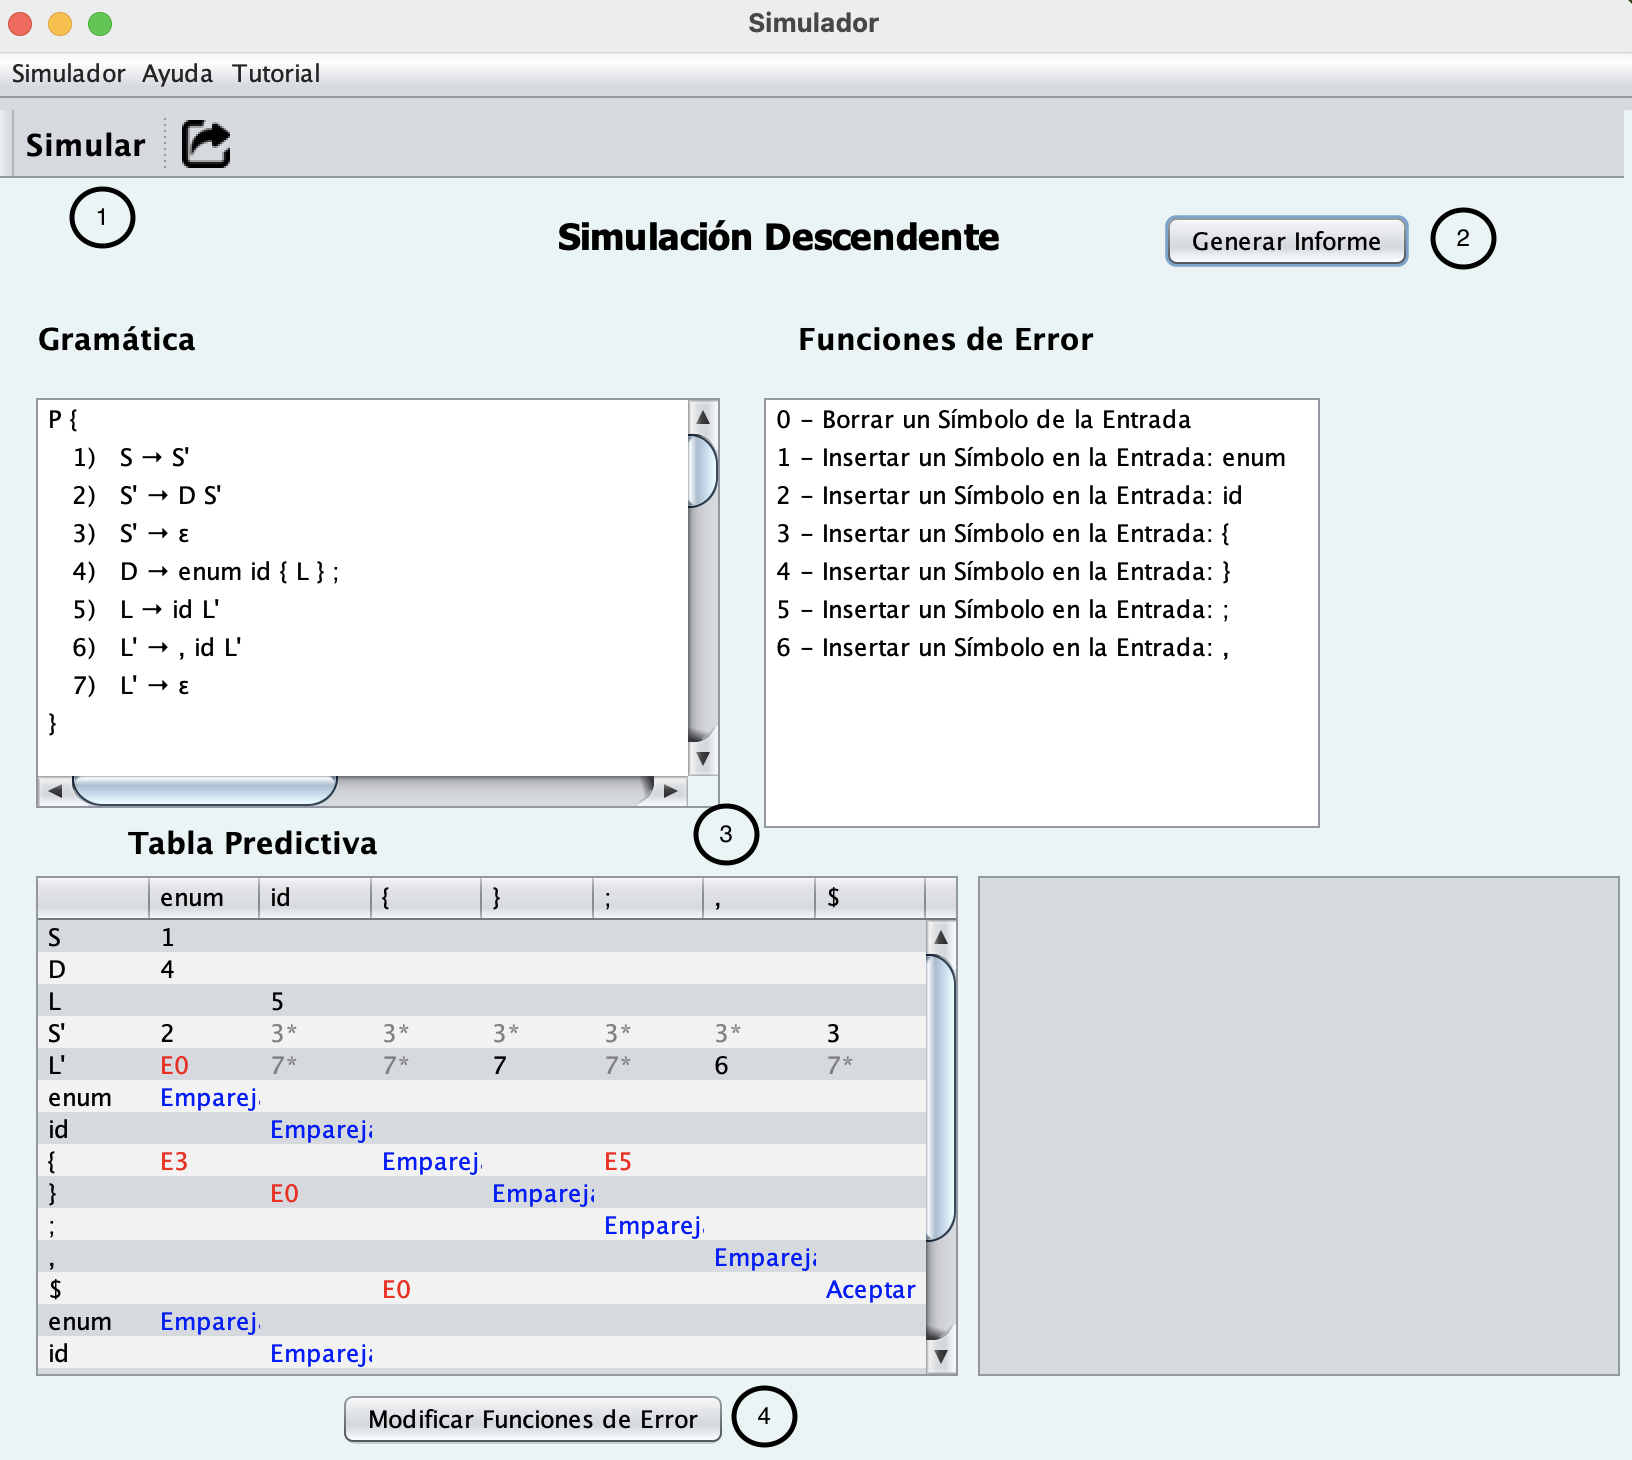
\includegraphics[scale=0.5]{figuras/Cap3/SimAS2/finalizar.png} 
       \caption{Tabla predictiva con funciones de errores de SimAS 2.0.}\label{fig:SimAS-2.0-finalizar}
 	\end{center}
\end{figure}

\newpage
La figura \ref{fig:SimAS-2.0-finalizar} muestra todo lo obtenido anteriormente respecto al análisis de las gramáticas en SimAS 2.0. En dicha figura, se han numerado algunos componentes que son descritos a continuación:
 \begin{enumerate}
     \item En primer lugar, nos da la posibilidad de realizar una simulación introduciendo algunos elementos de la gramática.
     \item En segundo lugar, se ofrece la posibilidad de generar un informe con todos los datos obtenidos en el análisis de la gramática.
     \item A continuación, se muestra un resumen con toda la información obtenida hasta el momento, como lo es la gramática sin recursividad, las funciones de error usadas y la tabla predictiva ya completa.
     \item Además, se tiene la opción de modificar las funciones de error que se han elegido con anterioridad.
 \end{enumerate}


\subsection{Fallos generales identificados en SimAS 2.0}

Durante el análisis y uso de la aplicación SimAS 2.0, se han identificado varios fallos y limitaciones que afectan a su funcionamiento y su utilidad como herramienta didáctica. A continuación, se detallan los fallos más relevantes:

\begin{enumerate}
    \item \textbf{Problemas en la persistencia de gramáticas:} al crear o modificar gramáticas en SimAS 2.0, se han observado ocasiones en las que los cambios realizados no se guardan correctamente en el sistema. Esto puede resultar en la pérdida de datos y en la necesidad de rehacer el trabajo. Por otro lado, cuando las gramáticas se guardan correctamente, la interpretación de los símbolos epsilon no se realiza de manera adecuada en algunos casos, lo que puede generar confusiones y errores en el análisis sintáctico.

    \item \textbf{Limitación en la generación de informes:} la funcionalidad de generación de informes presenta una limitación significativa, ya que solo se realiza correctamente en sistemas operativos Windows. En otros sistemas operativos, como Linux o macOS, la generación de informes puede fallar, lo que afecta la portabilidad y la usabilidad de la aplicación.
    
    \item \textbf{Problemas al añadir errores:} se ha observado que, en ciertas situaciones, al intentar agregar errores, la aplicación no permite su inserción en la parte de la tabla correspondiente, normalmente en la parte inferior. Este problema afecta la capacidad de los usuarios para simular y corregir errores sintácticos en gramáticas definidas.
    
    \item \textbf{Complejidad en la gestión de producciones gramaticales:} la gestión de producciones gramaticales, como añadir, modificar o eliminar producciones, presenta una complejidad innecesaria. Los usuarios encuentran dificultades al realizar estas operaciones, lo que afecta la eficiencia y la experiencia de uso de la aplicación.
    
    \item \textbf{Error ocasional en la generación de conjuntos Primero y Siguiente:} se han observado fallos intermitentes en el proceso de generación de conjuntos Primero y Siguiente. Estos conjuntos son fundamentales para varios algoritmos de análisis sintáctico, por lo que los errores en su cálculo pueden afectar a la precisión y la fiabilidad de la simulación.
    
    \item \textbf{Generación parcial de árboles de análisis:} actualmente, SimAS 2.0 no cuenta con la capacidad total de generar árboles sintácticos que representen las derivaciones realizadas durante el análisis sintáctico. El programa genera correctamente los árboles descendentes, excepto los nodos con el símbolo épsilon, y parcialmente los ascendentes en el sistema operativo Windows, pero, en otros sistemas operativos, no los genera bien. Esta funcionalidad es crucial para la comprensión visual del proceso de análisis y su ausencia limita el potencial educativo de la aplicación.
\end{enumerate}

La corrección y mejora de estos fallos son aspectos prioritarios para garantizar el correcto funcionamiento y la utilidad pedagógica de SimAS 2.0 como herramienta de aprendizaje en el ámbito del análisis sintáctico de lenguajes formales.

En la siguientes seccións, se profundizará con más detalle en los fallos encontrados para cada sistema operativo en el que se ha probado, ya que dependiendo de éste, la aplicación actúa de distinta forma.

Se va a utilizar la siguiente gramática de contexto libre para describir los fallos detectados en la apliación SimAS 2.0:
\begin{align*}
P = \{ & \\ 
S &\rightarrow S \, D \\
S &\rightarrow \varepsilon \\
D &\rightarrow T \, L \, ; \\
T &\rightarrow \text{REAL} \\
T &\rightarrow \text{ENTERO} \\
L &\rightarrow L \, , \, \text{ID} \\
L &\rightarrow \text{ID} \\
  & \}
\end{align*}

Esta es una gramática que genera declaraciones de variables tipo entero y real.

\subsection{Fallos encontrados en Windows}
Durante las pruebas realizadas en el sistema operativo Windows 11, se han identificado varios fallos en el funcionamiento de la aplicación SimAS. Uno de los problemas más destacados se refiere a la modificación de la gramática, tanto en los símbolos no terminales como en los símbolos terminales. Los usuarios encuentran dificultades al realizar operaciones como quitar o poner símbolos, así como al intentar renombrar un símbolo.

Además, se observaron inconsistencias en la validación de la gramática, lo que puede llevar a errores en la definición de la misma. Otro problema identificado está relacionado con la funcionalidad de guardar la gramática en el directorio correspondiente. En algunas ocasiones, la gramática no se guarda correctamente, lo que puede resultar en la pérdida de datos importantes para el usuario.

Durante las pruebas, también se identificaron fallos en la generación de los conjuntos Primero y Siguiente, que no se calculan de manera precisa. Esto puede afectar a la precisión de los análisis sintácticos realizados con la aplicación.

Además de los problemas mencionados anteriormente, se han detectado errores relacionados con la paginación del informe generado por la aplicación. La generación del árbol sintáctico para el símbolo épsilon también presenta problemas en algunas situaciones específicas.

Por último, se observó que al volver a acceder a la aplicación después de salir de la simulación descendente, los datos de la simulación anterior persisten de manera inesperada. Esto puede causar confusiones al usuario y afectar a la integridad de los resultados obtenidos.

\subsection{Fallos encontrados en Ubuntu}

En el entorno de Ubuntu 22, se han identificado varios problemas que afectan a la experiencia y funcionalidad de la aplicación SimAS.

Al eliminar un símbolo de la gramática y posteriormente intentar volver a añadirlo, se observa que es necesario cerrar la ventana emergente correspondiente y abrir una nueva para llevar a cabo la acción deseada. Esta situación puede resultar frustrante para el usuario, ya que interrumpe el flujo de trabajo y genera una experiencia poco fluida en la edición de la gramática.

Otro inconveniente detectado radica en el comportamiento al hacer clic repetidamente en la opción ``Visualizar Gramática Original''. En lugar de abrir la ventana una sola vez, se observa que la aplicación abre múltiples instancias de la ventana, lo cual puede resultar confuso para el usuario y generar una sensación de ineficiencia en la navegación por la interfaz, como se puede observar en la imagen \ref{fig:SimAS-2.0-ubuntu1}.

\begin{figure}[htp]
 	\begin{center}
      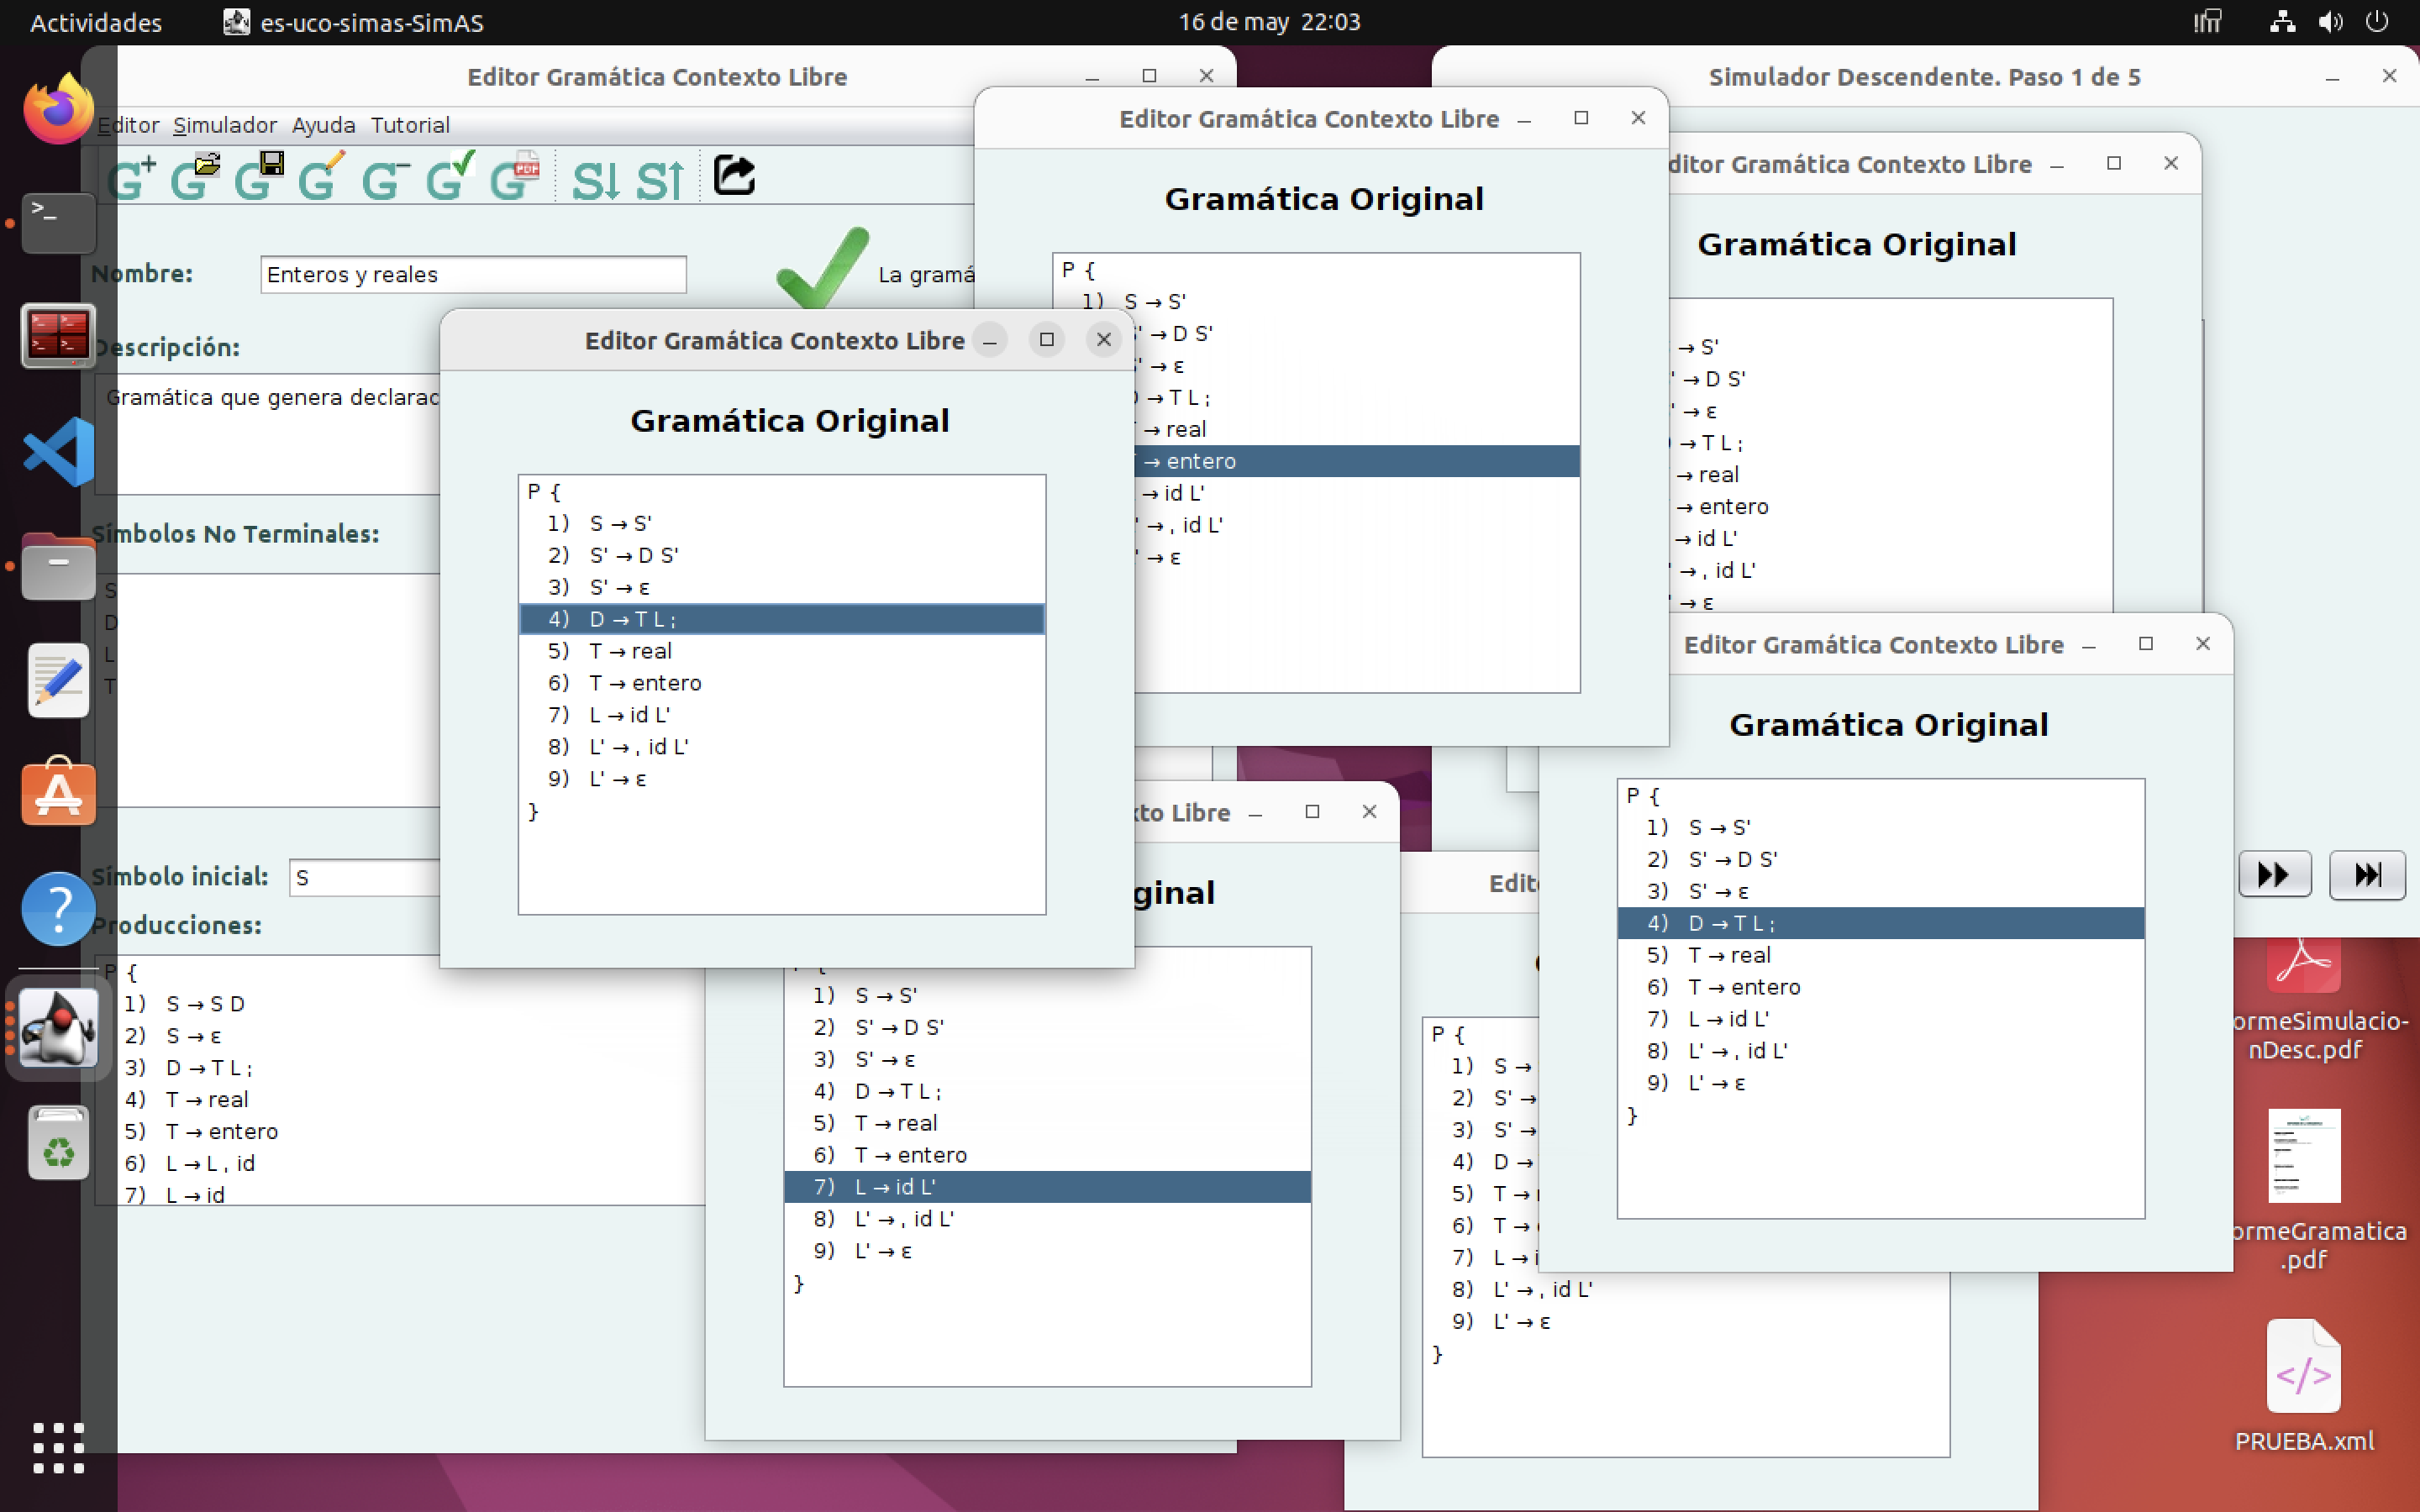
\includegraphics[scale=0.3]{figuras/Cap3/SimAS2/fallos/ubuntu1.png} 
       \caption{Generación repititiva de la visualización de la gramática}\label{fig:SimAS-2.0-ubuntu1}
 	\end{center}
\end{figure}

Además, se ha detectado que la aplicación no enumera las reglas al eliminar la recursividad en la gramática. Esta omisión puede dificultar la identificación y seguimiento de los cambios realizados en la estructura de la gramática, lo que puede conducir a errores o malentendidos durante el proceso de edición.

Otro problema importante afecta a la generación de los conjuntos Primero y Siguiente, los cuales no se calculan correctamente. Estos conjuntos son fundamentales para varios algoritmos de análisis sintáctico, por lo que errores en su cálculo pueden impactar negativamente en la precisión y fiabilidad de la simulación y validación de la gramática.

En relación con las funciones de error, se ha observado que la función de error para terminar el análisis no está predefinida, lo que puede dificultar la gestión de errores durante el análisis sintáctico y generar resultados inesperados.

Asimismo, al añadir una nueva regla de error, la aplicación no asigna automáticamente el siguiente número disponible, lo que puede generar confusiones en la gestión de las reglas de error y dificultar su identificación. En la figura \ref{fig:SimAS-2.0-ubuntu2} se observa la posibilidad de añadir cualquier número a las nuevas funciones de error, sin seguir ningún orden.

\begin{figure}[htp]
 	\begin{center}
      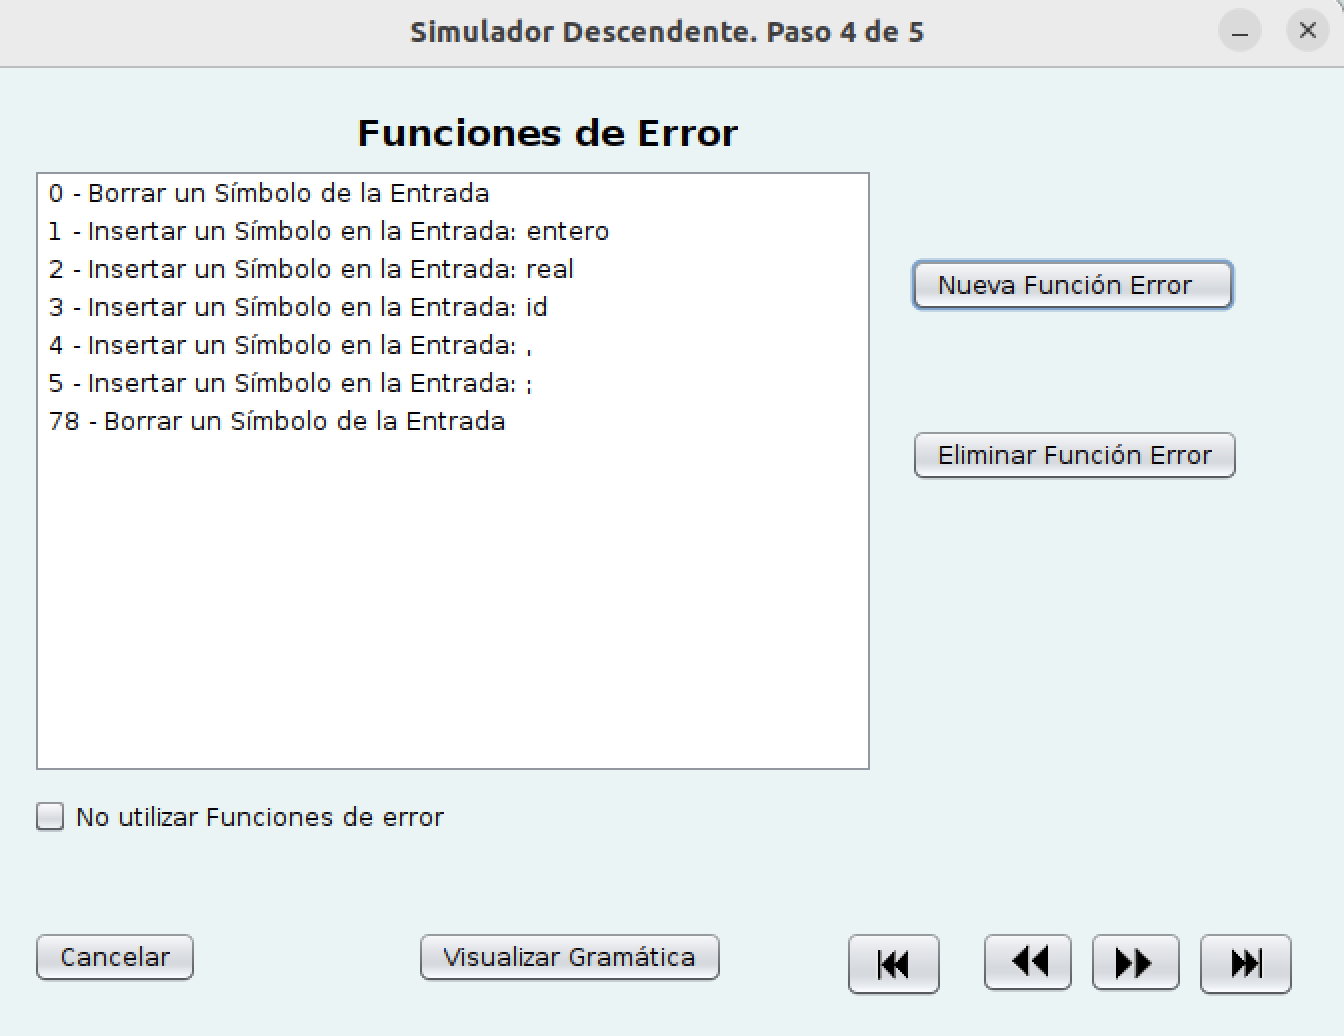
\includegraphics[scale=0.3]{figuras/Cap3/SimAS2/fallos/ubuntu2.png} 
       \caption{Creación de una nueva función de error}\label{fig:SimAS-2.0-ubuntu2}
 	\end{center}
\end{figure}

Otro problema destacable ocurre al intentar modificar las funciones de error después de haber finalizado y regresado al proceso. En esta situación, la aplicación duplica las filas de los símbolos terminales y modifica los estados de la tabla predictiva, lo que puede causar errores en la definición y gestión de las funciones de error.

La generación incorrecta de informes de simulación descendente y la ausencia de generación de informes tras realizar un análisis de una cadena de entrada también se han identificado como fallos significativos en el funcionamiento de la aplicación en el entorno de Ubuntu 22. Estos problemas afectan negativamente a la capacidad del usuario para evaluar y analizar los resultados del análisis sintáctico, lo que impacta en la utilidad y fiabilidad de la aplicación en este sistema operativo.

\subsection{Fallos encontrados en MacOS}

Al crear una nueva gramática, el programa no proporciona una opción para regresar al menú principal, lo que dificulta la navegación dentro de la aplicación. Además, al validar una gramática, se abren dos ventanas emergentes, una con la gramática validada y otra que queda congelada, lo que puede resultar confuso para el usuario, observable en la figura \ref{fig:SimAS-2.0-macos1}. Por otro lado, al intentar copiar y pegar texto al agregar o modificar símbolos de la gramática, así como al cambiar el nombre de los símbolos, la funcionalidad no está habilitada, lo que limita la capacidad del usuario para editar la gramática de manera eficiente.

\begin{figure}[htp]
 	\begin{center}
      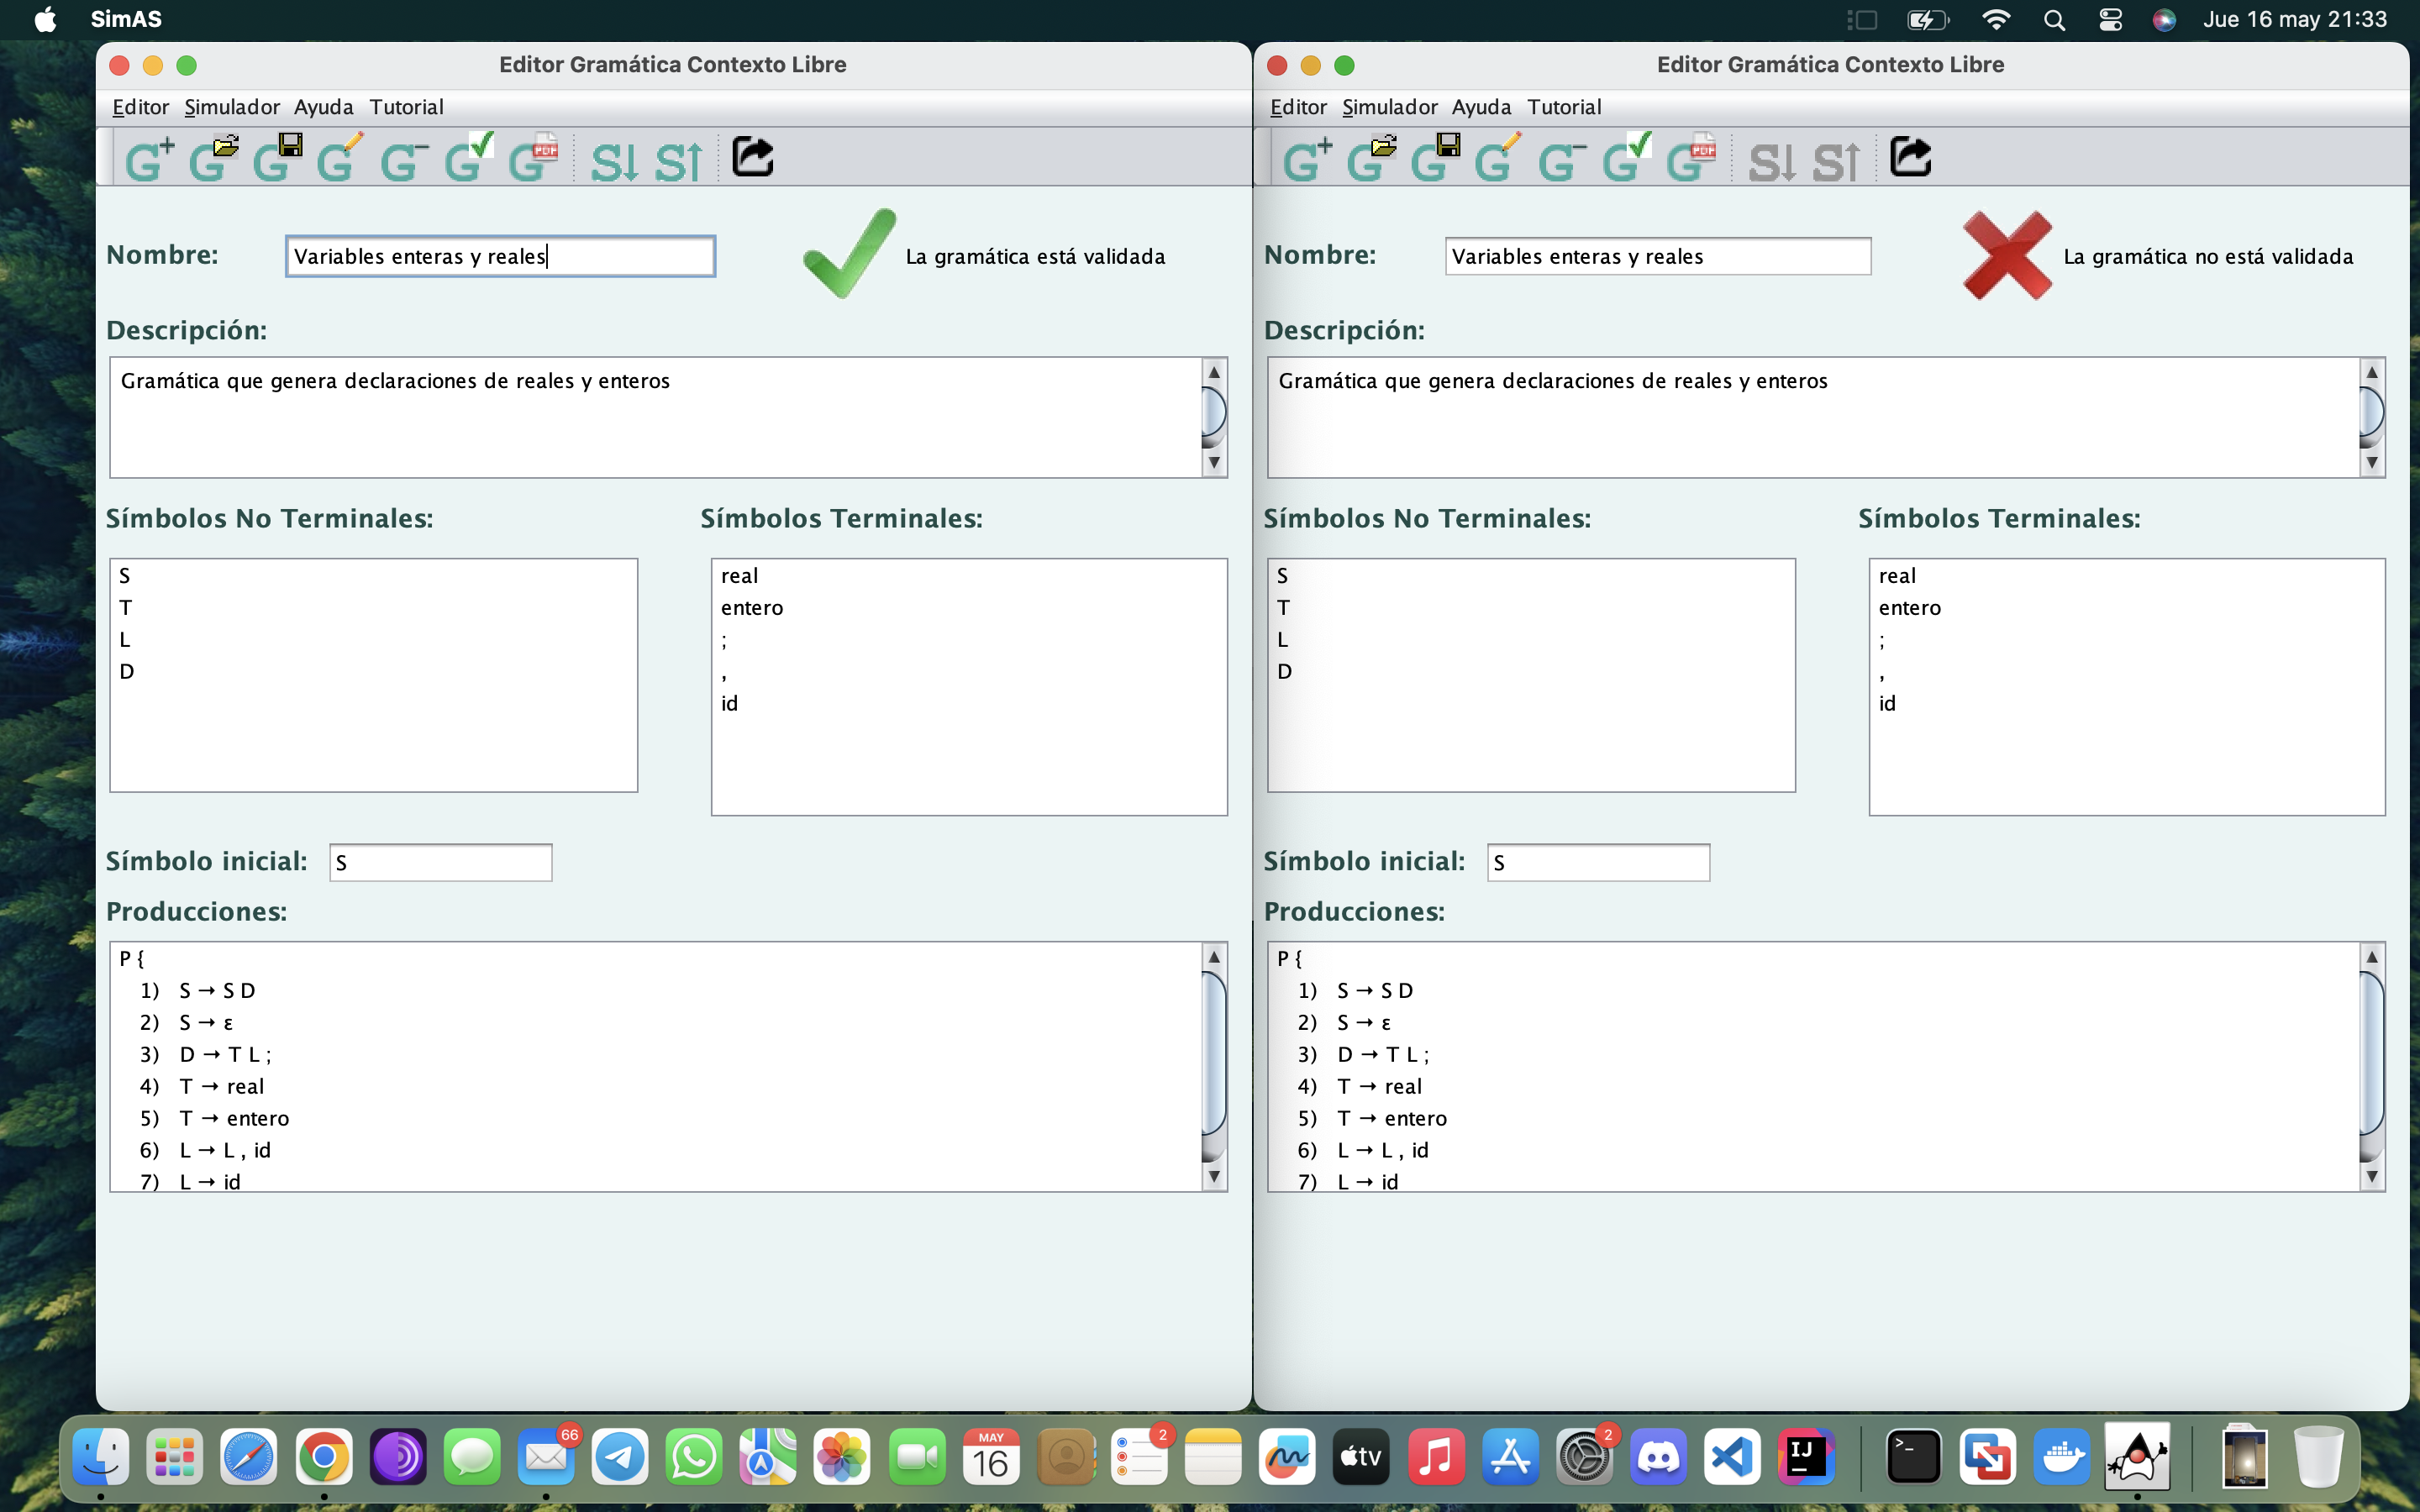
\includegraphics[scale=0.3]{figuras/Cap3/SimAS2/fallos/macos1.png} 
       \caption{Abrir gramática en MacOS.}\label{fig:SimAS-2.0-macos1}
 	\end{center}
\end{figure}

La aplicación no permite numerar las reglas de la gramática, lo que dificulta la identificación y referencia de las reglas durante el proceso de desarrollo. Asimismo, la imposibilidad de cambiar el orden de las reglas gramaticales puede causar problemas al corregir errores o reorganizar la estructura de la gramática.

En ciertas situaciones, el programa no incluye automáticamente la función de terminar el análisis en la tabla de funciones de error, lo que puede afectar la experiencia del usuario al simular la gramática. Además, al agregar una nueva regla de error, no se asigna automáticamente el siguiente número disponible, lo que puede resultar en la duplicación de números de reglas y generar confusión en la identificación de errores.

El informe generado por la aplicación no se visualiza correctamente en macOS, ya que al intentar abrirlo aparece un error al cargar el documento PDF. Este problema afecta la capacidad del usuario para revisar y analizar los resultados de la simulación de manera efectiva.

Al intentar modificar las funciones de error en la tabla predictiva, el programa duplica los símbolos no terminales en las filas y cambia los estados de la tabla predictiva, como se puede ver enla imagen \ref{fig:SimAS-2.0-macos2}. Este comportamiento inesperado puede causar errores en la interpretación de la tabla y afectar la precisión del análisis sintáctico.

\begin{figure}[htp]
 	\begin{center}
      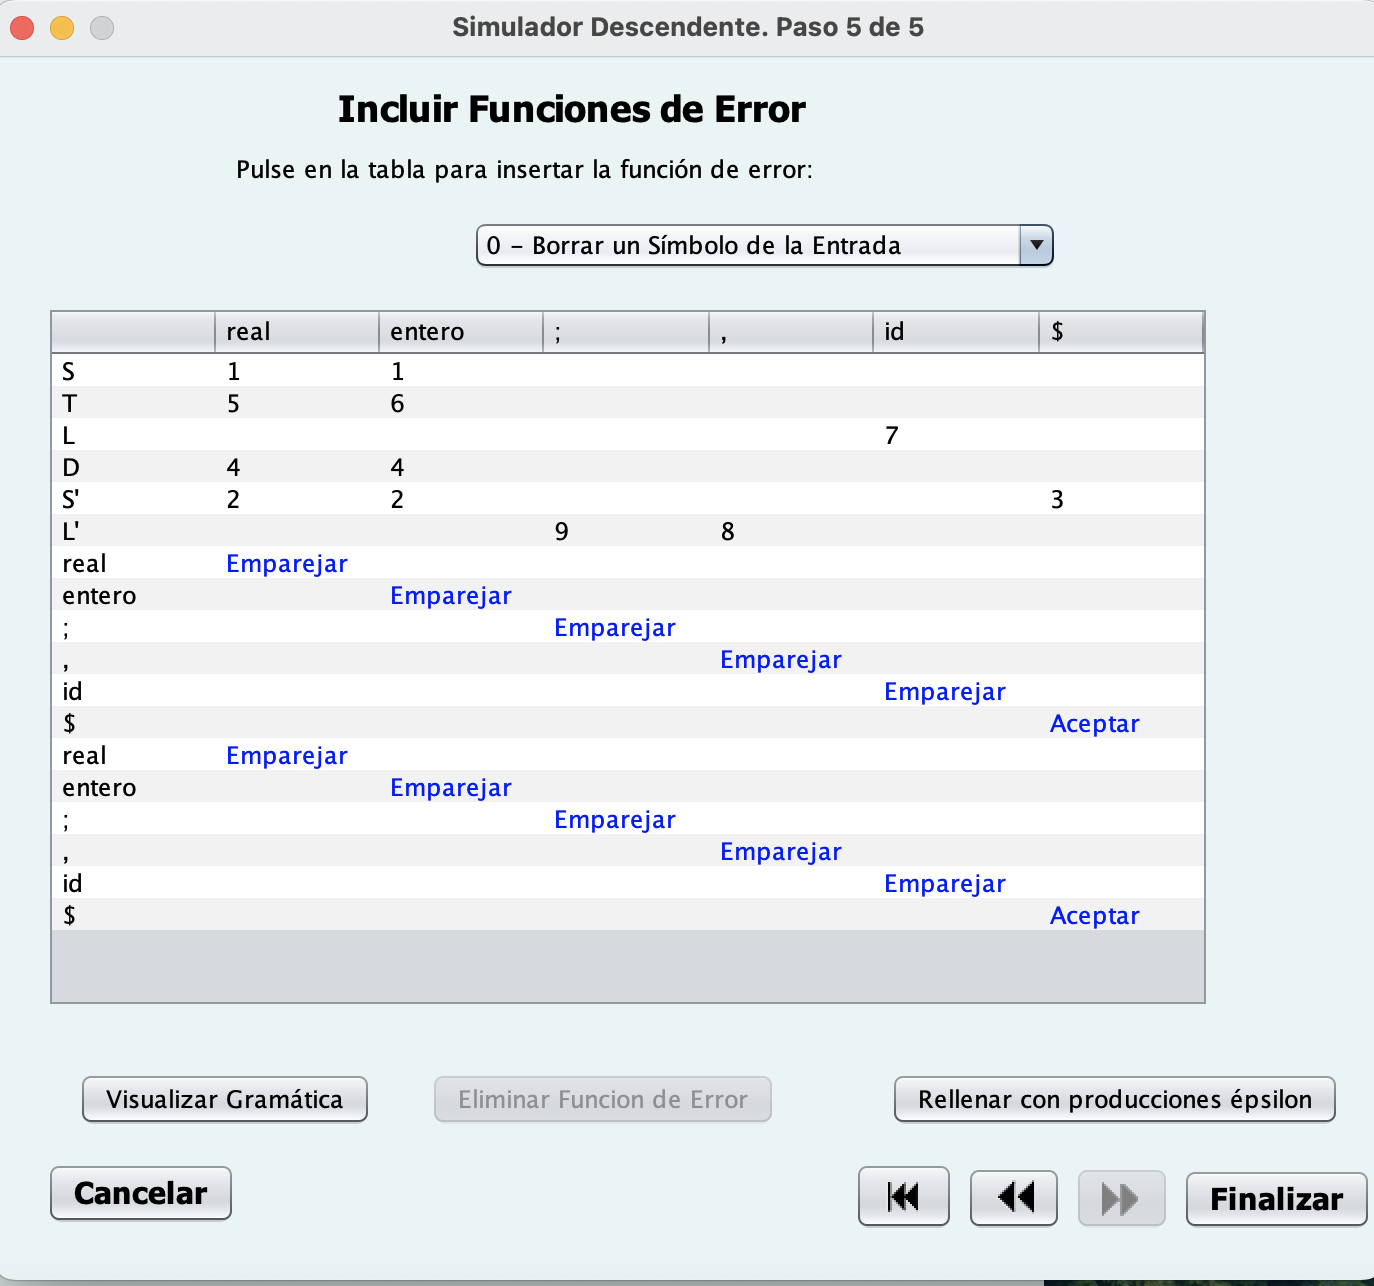
\includegraphics[scale=0.5]{figuras/Cap3/SimAS2/fallos/macos2.png} 
       \caption{Duplicación símbolos no terminales MacOS}\label{fig:SimAS-2.0-macos2}
 	\end{center}
\end{figure}

Durante la simulación descendente, la aplicación no permite incluir la cadena de entrada, lo que limita la capacidad del usuario para probar diferentes cadenas de entrada y verificar la precisión del análisis sintáctico. Además, al realizar la simulación descendente y agregar la declaración, la ventana emergente no se cierra automáticamente al aceptar la acción, lo que puede resultar en una experiencia de usuario inconsistente y confusa.


%Cambiar mayusculas por minusculas despues de :
\section{Justificación del trabajo} \label{sec:justificacion}

El desarrollo del presente Trabajo de Fin de Grado está justificado porque puede mejorar la versión anterior de la aplicación SimAS 2.0 \cite{juan}, que a su vez es una evolución de la primera versión desarrollada anteriormente \cite{vanesa}. Esta justificación se fundamenta en varios aspectos relevantes:

\begin{enumerate}
    \item \textbf{Corrección de problemas detectados}: la detección de algunos problemas y limitaciones en la versión anterior de SimAS 2.0 ha evidenciado la necesidad de realizar mejoras significativas. Estos problemas han obstaculizado el aprendizaje completo de los análisis sintácticos ascendentes y descendentes, lo que motiva la búsqueda de soluciones efectivas.
    
    \item \textbf{Mejora del aprendizaje interactivo}: se espera que la mejora y corrección de la aplicación conduzca a un funcionamiento más completo y correcto, lo que facilitará el aprendizaje profundo de los conceptos relacionados con los análisis sintácticos. Este enfoque interactivo no solo beneficia a los estudiantes, sino que también puede ser una herramienta valiosa para los profesores en la enseñanza de la asignatura de Procesadores de Lenguajes.
    
    \item \textbf{Impacto en el ámbito educativo y académico}: el desarrollo de una herramienta de aprendizaje interactiva como SimAS 3.0 tiene el potencial de tener un impacto significativo en el ámbito educativo y académico. Proporciona una oportunidad para mejorar la comprensión y el dominio de conceptos complejos en el campo de la informática, especialmente en lo relacionado con el procesamiento de lenguajes.
    
    \item \textbf{Continuidad y evolución del proyecto}: al seguir la evolución del proyecto desde la versión original hasta la actual, se establece una continuidad en la mejora y perfeccionamiento de la aplicación. Esta progresión refleja un compromiso constante con la excelencia y la adaptación a las necesidades cambiantes de los usuarios y del entorno educativo.
    
    \item \textbf{Facilitación del aprendizaje mediante una interfaz intuitiva}: la implementación de una interfaz más intuitiva y amigable con el usuario tiene como objetivo principal hacer que el proceso de aprendizaje sea más accesible y efectivo para los estudiantes. Esta mejora se alinea con las tendencias actuales en el diseño de herramientas educativas, que buscan maximizar la usabilidad y la experiencia del usuario.

    \item \textbf{Innovación y avance tecnológico}: la mejora y actualización de SimAS 3.0 representa un avance en la aplicación de nuevas tecnologías y metodologías en el campo de la educación informática. Este enfoque innovador busca aprovechar al máximo las capacidades de las herramientas digitales para mejorar la calidad y efectividad del aprendizaje.

    \item \textbf{Fomento del desarrollo profesional}: la participación en este proyecto brinda la oportunidad de adquirir y desarrollar habilidades técnicas y profesionales relevantes, como el diseño de software, la programación en Java y el trabajo en equipo. Estas habilidades son altamente valoradas en el mercado laboral y contribuyen al crecimiento profesional del estudiante.
    
    \item \textbf{Contribución a la comunidad académica}: al compartir los resultados y el código fuente de SimAS 3.0, se contribuye al conocimiento colectivo y se fomenta la colaboración entre instituciones educativas y profesionales del campo de la informática. Esta contribución puede dar lugar a nuevas investigaciones y desarrollos en el área de los procesadores de lenguajes y la educación informática en general.
    
    \item \textbf{Relevancia y aplicabilidad práctica}: la aplicación de SimAS 3.0 no solo se limita al ámbito académico, sino que también tiene aplicaciones prácticas en la industria y el desarrollo de software. La comprensión profunda de los análisis sintácticos que proporciona la herramienta es fundamental para el diseño y la implementación de compiladores y otros sistemas de procesamiento de lenguajes en la práctica profesional.

\end{enumerate}

En resumen, la realización de este trabajo se justifica por la necesidad de mejorar y perfeccionar una herramienta educativa clave en el ámbito de la informática, con el fin de proporcionar una experiencia de aprendizaje más efectiva y enriquecedora para los estudiantes.


\subsection{Comparativa entre versiones}
La Tabla \ref{tlb:tabla3_1} muestra, brevemente, una comparativa de las versiones 1.0 y lo que se pretendió alcanzar con la nueva versión 2.0 de SimAS, además de una comparativa con las características esperadas en la nueva versión, ``SimAS 3.0 descendente preditivo''. 

%Revisar tabla
\begin{center}
 \begin{table}[H]
 \caption{Comparación entre versiones de SimAS.}\label{tlb:tabla3_1}
 \resizebox{15cm}{!} 
 {
 \begin{tabular}[c]{| l | c | c | c |}
 \hline
   & \textbf{SimAS 1.0} & \textbf{SimAS 2.0} & \textbf{SimAS 3.0}  \\ 
   &   & & \textbf{descendente predictivo}  \\ \hline
  Edición de gramáticas de contexto libre & Sí & Sí & Sí  \\ \hline
  Análisis sintáctico descendente & Sí & Sí & Sí  \\ \hline
  Análisis sintáctico ascendente & Sí & Sí & No \\ \hline
  Generación de árboles sintácticos & No & Parcial & Sí  \\ \hline
  Generación de informes & No & Parcial & Sí \\ \hline
  Definición de funciones predefinidas & \multirow{2}*{No}  & \multirow{2}*{Parcial} & \multirow{2}*{Sí}   \\ 
   de tratamiento de errores &  &  &  \\ \hline 
   Compatibilidad multiplataforma & Parcial & Parcial & Sí \\ \hline
 \end{tabular}
 }
 \end{table}
\end{center}